%!TEX root = ../thesis.tex
%*******************************************************************************
%*********************************** Results *********
%*******************************************************************************


\chapter{Results}\label{ch:results}

\ifpdf
    \graphicspath{{chapter-results/Figs/Raster/}{chapter-results/Figs/PDF/}{chapter-results/Figs/}}
\else
    \graphicspath{{chapter-results/Figs/Vector/}{chapter-results/Figs/}}
\fi

This chapter discusses the results of the different fit configurations and hypothesis tests performed in the analysis. After the background estimation obtained through a background-only fit in the \glspl{cr} is validated in the \glspl{vr}, the \glspl{sr} are unblinded and the observed data is compared to the \gls{sm} background expectation.

\section{Background-only fit results}\label{sec:results_background_only}

\subsection{Results in the control regions}

 \begin{figure}
	\centering
	\begin{subfigure}[b]{0.5\linewidth}
		\centering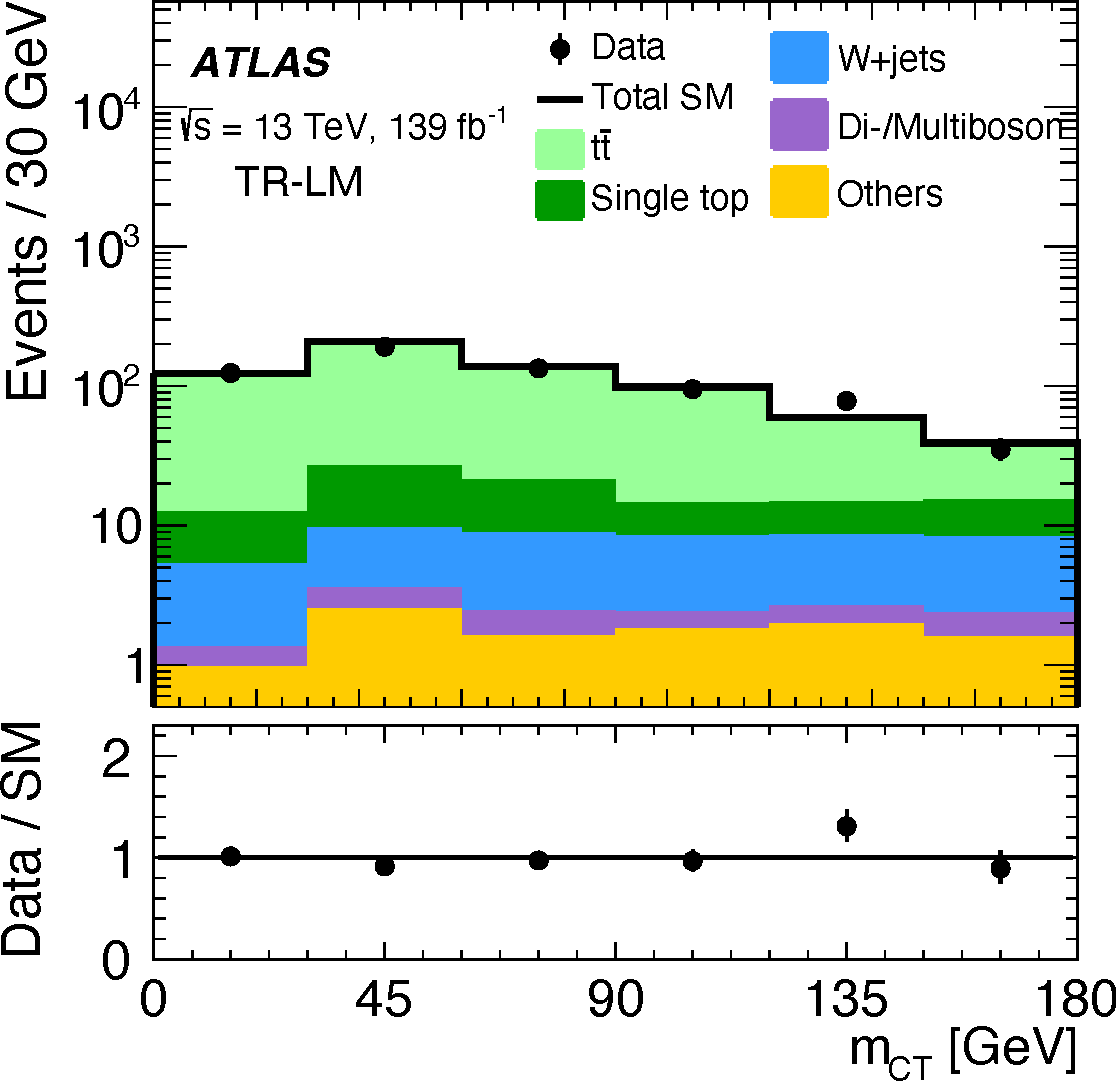
\includegraphics[width=0.85\textwidth]{OneLeptonbb_CR_TRLMEM_mct2_yellow}
	\end{subfigure}\hfill
	\begin{subfigure}[b]{0.5\linewidth}
		\centering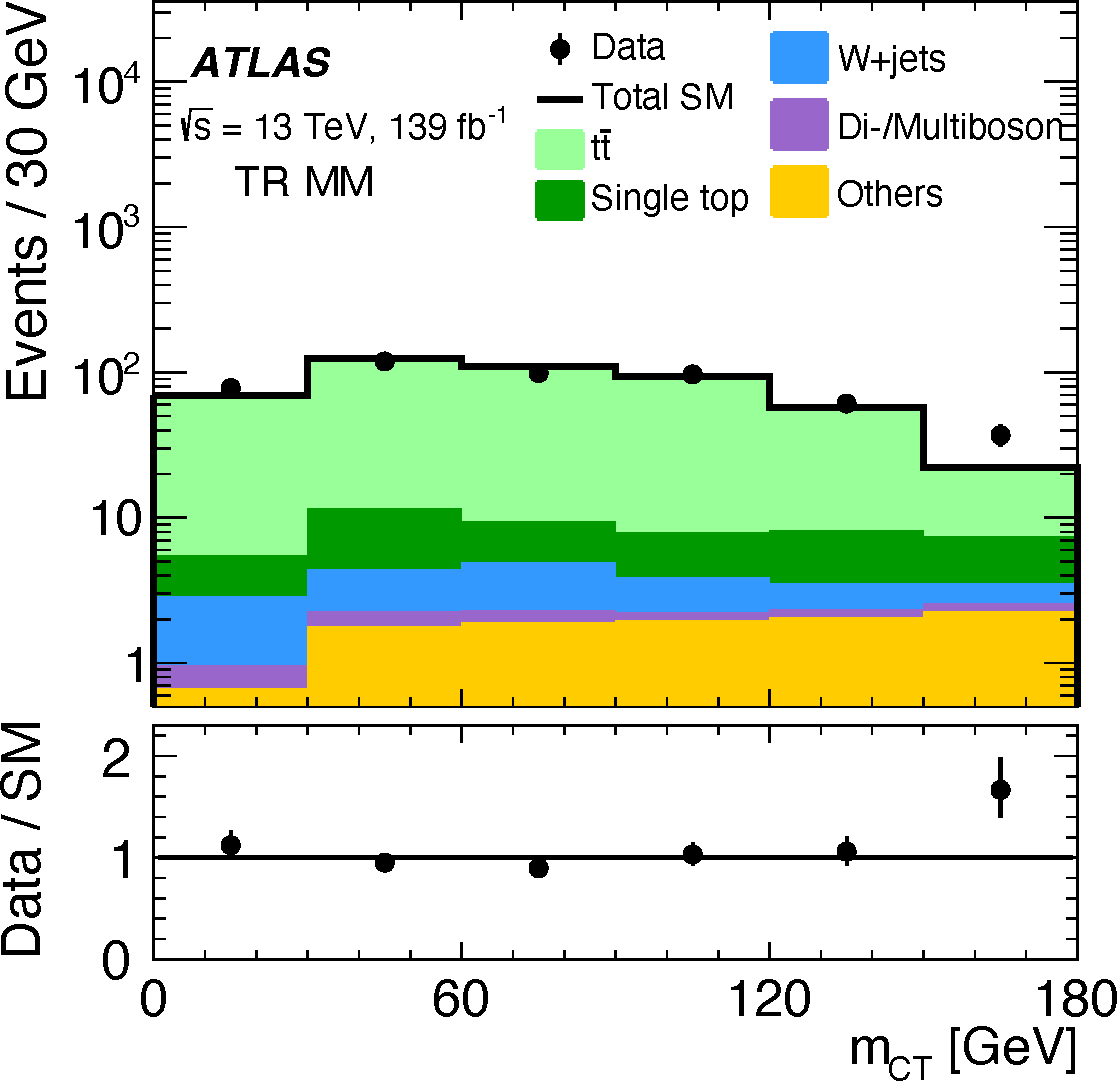
\includegraphics[width=0.85\textwidth]{OneLeptonbb_CR_TRMMEM_mct2_yellow}
	\end{subfigure}\hfill
	\par\medskip
	\begin{subfigure}[b]{0.5\linewidth}
		\centering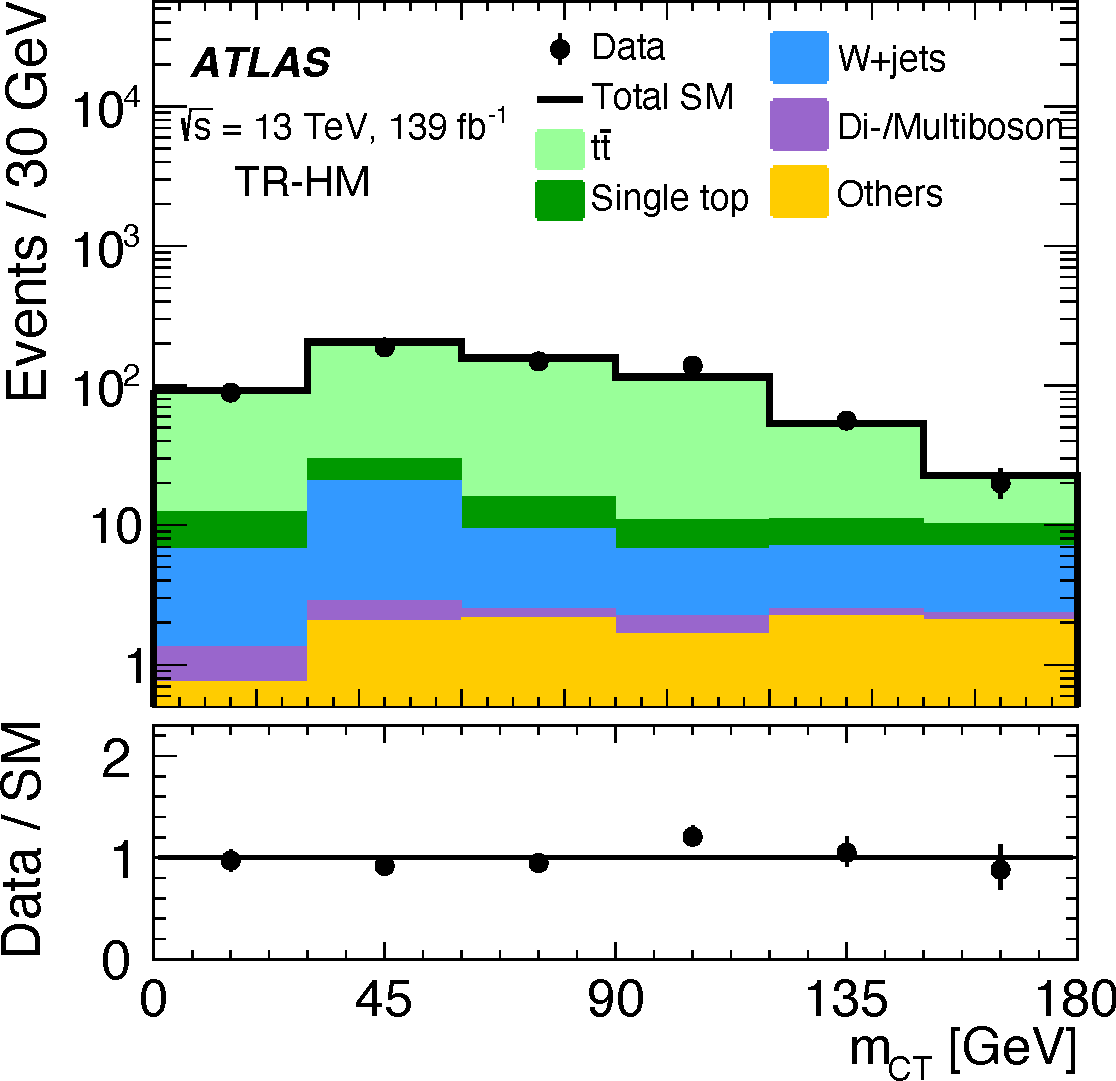
\includegraphics[width=0.85\textwidth]{OneLeptonbb_CR_TRHMEM_mct2_yellow}
	\end{subfigure}\hfill
	\begin{subfigure}[b]{0.5\linewidth}
		\centering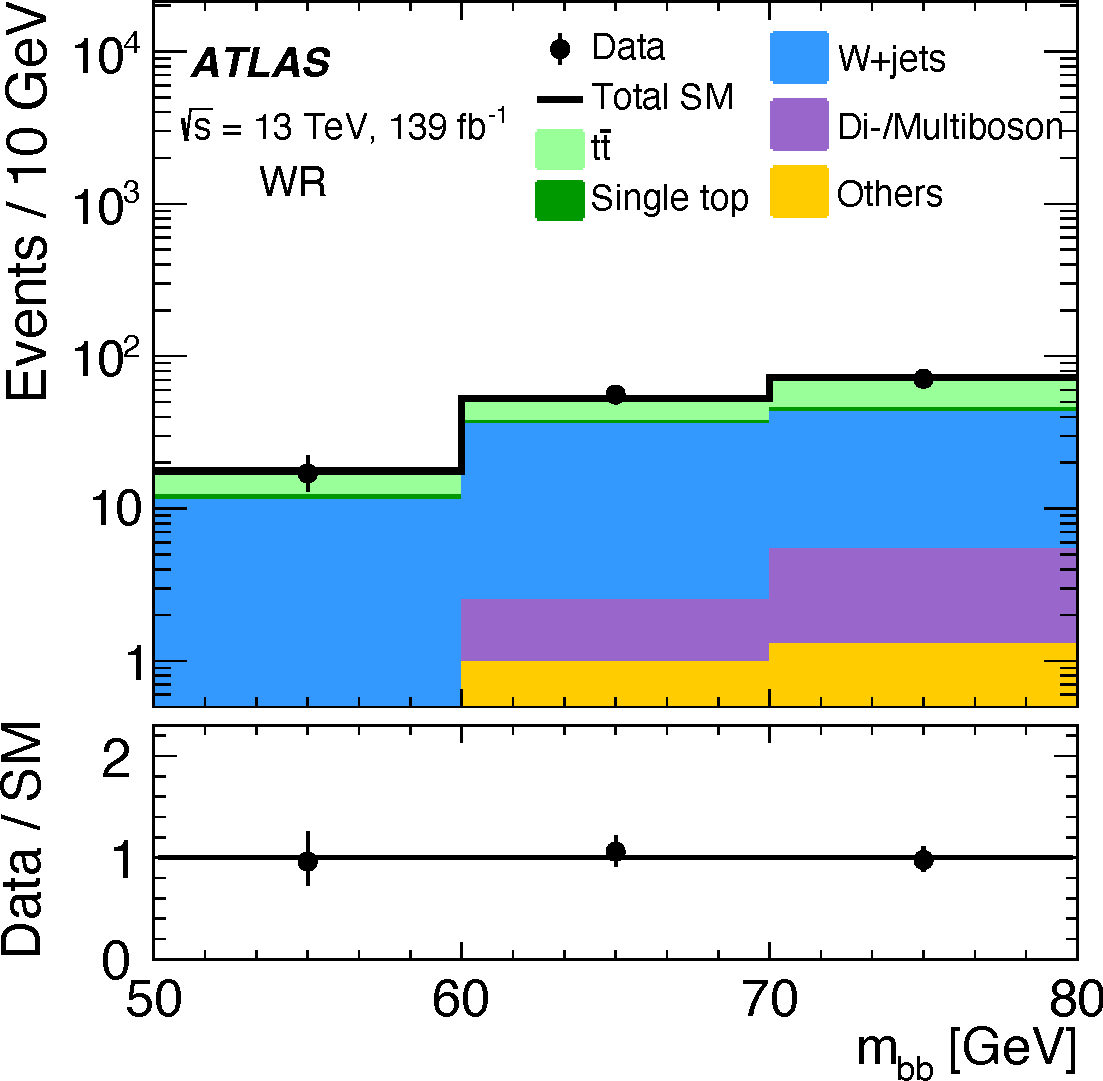
\includegraphics[width=0.85\textwidth]{OneLeptonbb_CR_WREM_mbb_yellow}
	\end{subfigure}\hfill
	\par\medskip
	\begin{subfigure}[b]{0.5\linewidth}
		\centering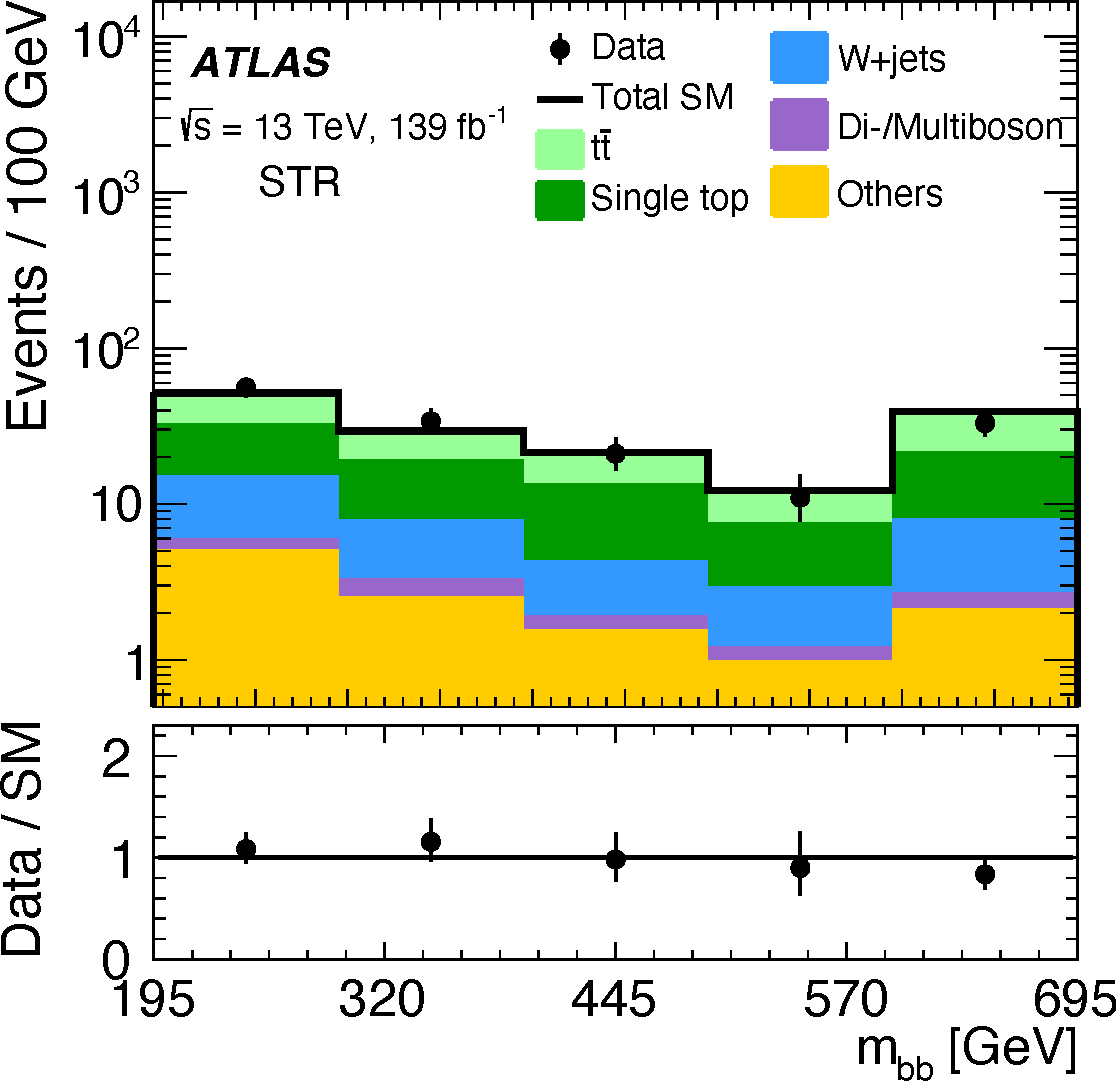
\includegraphics[width=0.85\textwidth]{OneLeptonbb_CR_STCREM_mbb_yellow}
	\end{subfigure}\hfill

	\caption{Exemplary distribution shown in each control region after the background-only fit. The shaded region includes all systematic uncertainties as well as \gls{mc} statistical uncertainty. The $\ttbar$, single top and $\wjets$ are normalised simultaneously in all \glspl{cr}. A good agreement between \gls{mc} expectation and data is observed in all \glspl{cr}.}
	\label{fig:CR_distributions_postfit}
\end{figure}



\begin{table}
\begin{center}
{\small
%%
\begin{tabular}{lrrrrr}
\toprule
Region           & TR-LM            & TR-MM            & TR-HM            & WR            & STCR              \\[-0.05cm]
\midrule
%%
Observed events          & $657$              & $491$              & $641$              & $144$              & $155$                    \\
\midrule
%%
Fitted SM events         & $666 \pm 25$          & $480 \pm 21$          & $645 \pm 26$          & $143 \pm 12$          & $154 \pm 15$              \\
\noalign{\smallskip}\hline\noalign{\smallskip}
%%
        $\ttbar$         & $560 \pm 40$          & $430 \pm 33$          & $550 \pm 40$          & $47 \pm 9$          & $59 \pm 12$              \\
%%
        Single top         & $60 \pm 40$          & $27 \pm 23$          & $33 \pm 27$          & $5 \pm 4$          & $57 \pm 22$              \\
%%
        $\wjets$         & $34 \pm 8$          & $10.5 \pm 2.8$          & $44 \pm 11$          & $83 \pm 16$          & $23 \pm 6$              \\
%%
        Di-/Multiboson        & $4.3 \pm 1.2$          & $2.0 \pm 0.5$          & $2.8 \pm 0.5$          & $5.7 \pm 1.0$          & $2.8 \pm 0.9$              \\
%%
        Other       & $10.5 \pm 1.3$          & $10.6 \pm 1.4$          & $11.1 \pm 1.4$          & $2.4 \pm 0.4$          & $12.3 \pm 1.5$              \\
%%     
\toprule
%%
MC exp. SM events              & $720 \pm 80$          & $474 \pm 33$          & $680 \pm 50$          & $130 \pm 13$          & $180 \pm 50$              \\
\midrule
%%
        $\ttbar$        & $570 \pm 70$          & $407 \pm 30$          & $570 \pm 40$          & $46 \pm 10$          & $52 \pm 10$              \\
%%
        Single top         & $102 \pm 18$          & $46 \pm 13$          & $58 \pm 16$          & $9 \pm 6$          & $90 \pm 40$              \\
%%
        $\wjets$         & $29 \pm 4$          & $8.4 \pm 1.2$          & $36.1 \pm 3.1$          & $67 \pm 5$          & $19.0 \pm 2.0$              \\
%%
        Di-/Multiboson         & $4.1 \pm 1.1$          & $2.0 \pm 0.5$          & $2.8 \pm 0.5$          & $5.6 \pm 1.0$          & $2.8 \pm 0.9$              \\
%%
       Other        & $10.6 \pm 1.3$          & $10.6 \pm 1.4$          & $11.2 \pm 1.4$          & $2.5 \pm 0.4$          & $12.4 \pm 1.5$              \\
%%     \\
\bottomrule\end{tabular}
%%%%
}
\end{center}
\caption{ Background-only fit results for the \glspl{cr} for an integrated luminosity of \onethirtynineifb. Nominal MC expectations (normalised to MC cross-sections) are given for comparison. The errors shown include the \gls{mc} statistical and systematic uncertainties.
%PDG rounding is applied to the event rates and uncertainties~\cite{pdg2020}.
}
\label{tab:results_bkg_only_CR}
\end{table}
%

As all \glspl{cr} are mutually exclusive, a background-only fit simultaneously using information from all \glspl{cr} can be run. Only the terms for the \glspl{cr} enter the likelihood as channels and any signal contamination present in the \glspl{cr} is neglected. This allows to fit the dominant backgrounds to data, and thus, by construction, leads to a good agreement between observed data and the total fitted background estimate in all \glspl{cr}. The free normalisation parameters for $\ttbar$ ($\mu_\mathrm{T}$), single top ($\mu_\mathrm{ST}$) and $\wjets$ ($\mu_\mathrm{W}$) are fitted to be
\begin{equation}
	\begin{split}
		\mu_\mathrm{T} = 1.02^{+0.07}_{-0.09}, \\
		\mu_\mathrm{ST} = 0.6^{+0.5}_{-0.25}, \\
		\mu_\mathrm{W} = 1.22^{+0.26}_{-0.24}. \\
	\end{split}
\end{equation}
While the dominant $\ttbar$ background stays roughly at its nominal expectation with respect to \gls{mc} simulation, $\wjets$ processes are scaled up, and the single top expectation is scaled down. The high uncertainty on $\mu_\mathrm{ST}$ can be attributed to the relatively low \gls{mc} statistics and comparably low purity of single top events in STR.

\Cref{tab:results_bkg_only_CR} summarises the fitted background estimate including all uncertainties for all control regions. As discussed in~\cref{ch:background_estimation}, $\ttbar$ is the most dominant in all control regions except WR where $\wjets$ is the largest background, followed by single top and $\wjets$ processes. Due to the relatively small normalisation factor for single top processes, $\ttbar$ and single top contribute to roughly equal amounts to STCR. Small contributions come from diboson, multiboson as well as other backgrounds like $\ttbar+V$, $\ttbar+h$ and $V+h$. All processes estimated directly from \gls{mc} simulation cumulatively account for only 10\%, 5.5\% and a maximum of 2.6\% in the single top, $\wjets$ and $\ttbar$ control regions, respectively. Exemplary distributions in the \glspl{cr} after the background-only fit are shown in~\cref{fig:CR_distributions_postfit}, revealing a good agreement between observed data and the \gls{sm} background estimate throughout the distributions shown.

\subsection{Results in the validation regions}
	
 \begin{figure}
	\centering
	\begin{subfigure}[b]{0.5\linewidth}
		\centering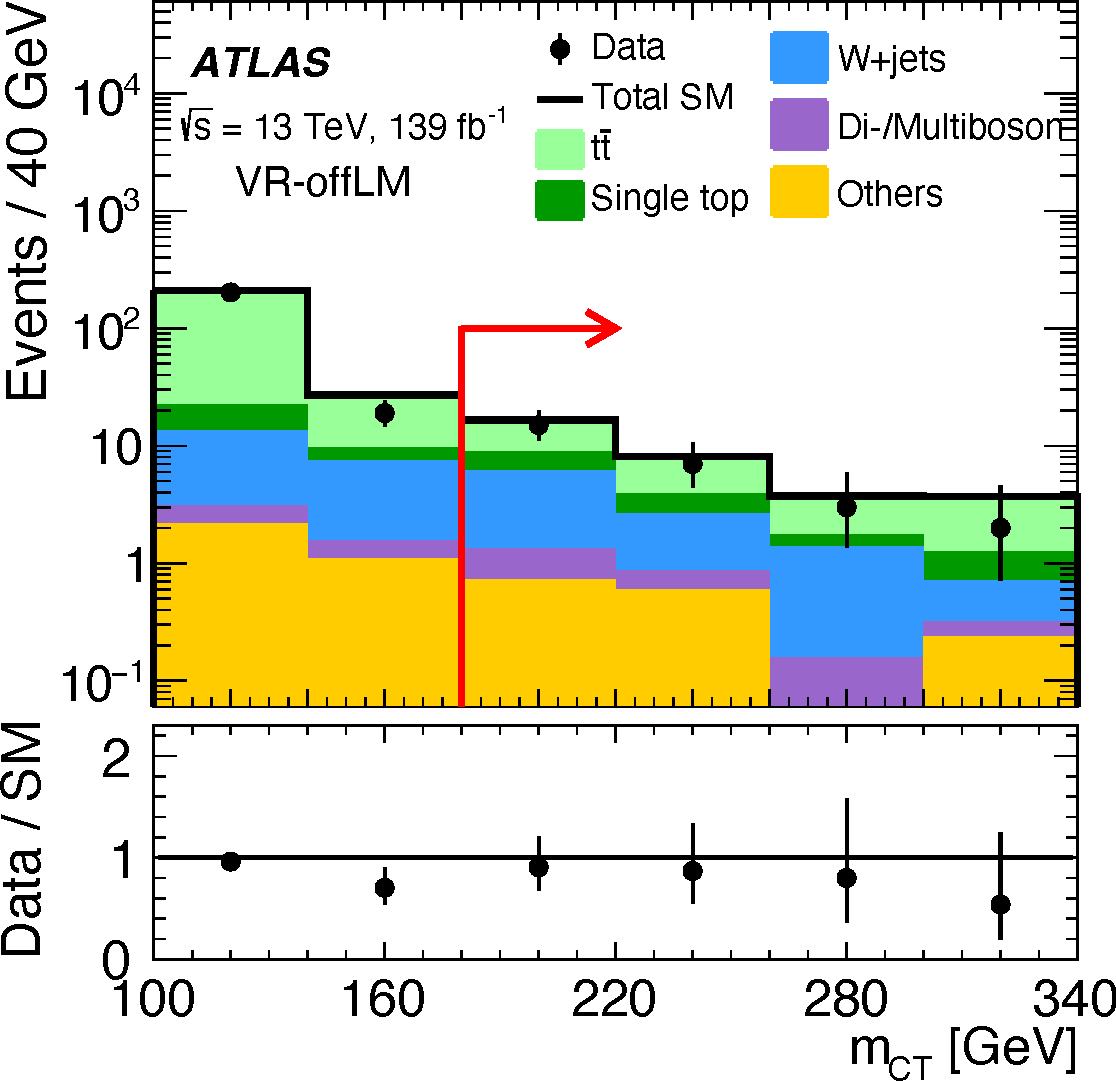
\includegraphics[width=0.85\textwidth]{OneLeptonbb_VR_UnderFlowBin_VRtt1offnomct2EM_mct2_yellow}
	\end{subfigure}\hfill
	\begin{subfigure}[b]{0.5\linewidth}
		\centering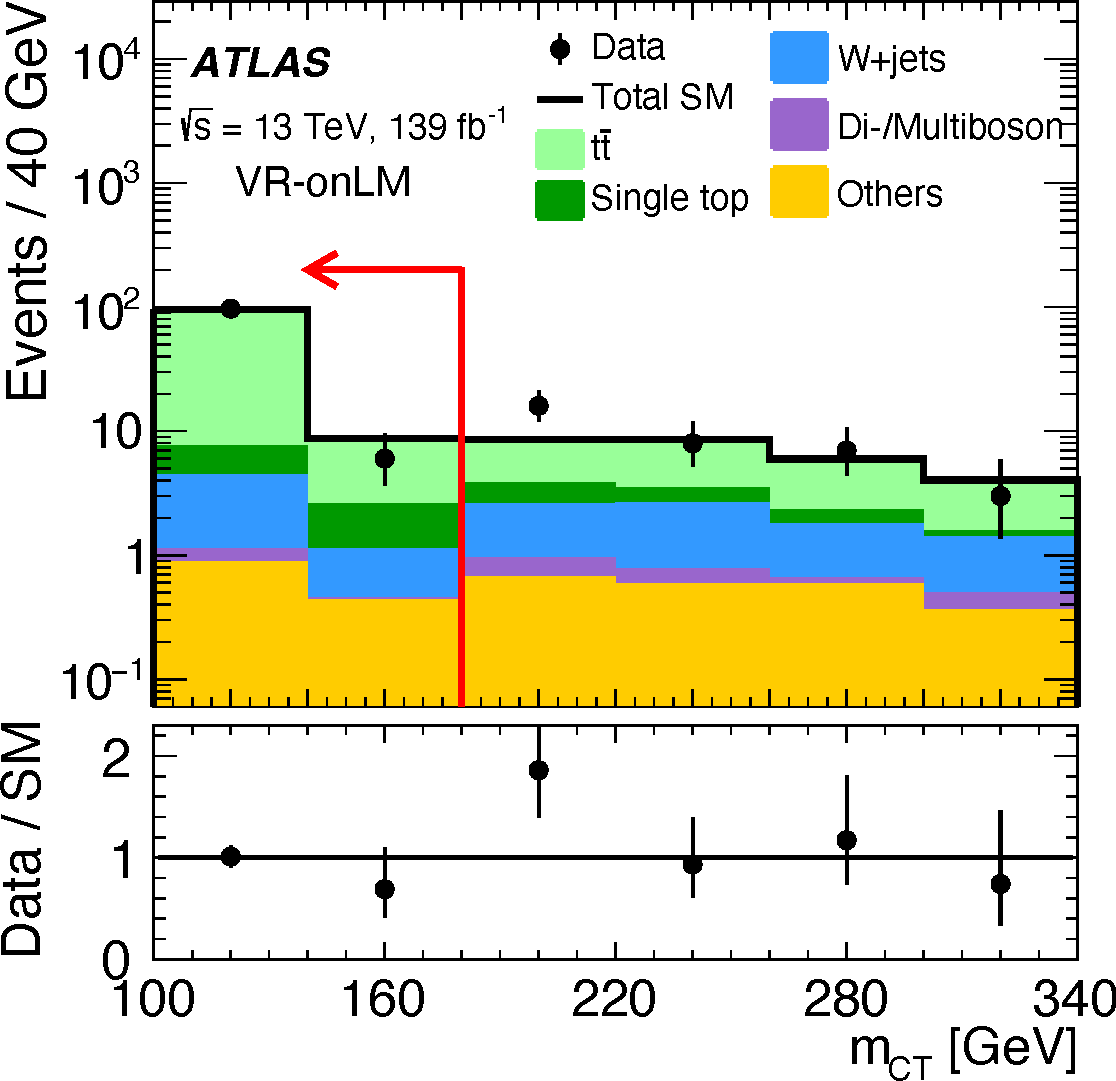
\includegraphics[width=0.85\textwidth]{OneLeptonbb_VR_UnderFlowBin_VRtt1onnomct2EM_mct2_yellow}
	\end{subfigure}\hfill
	\par\medskip
	\begin{subfigure}[b]{0.5\linewidth}
		\centering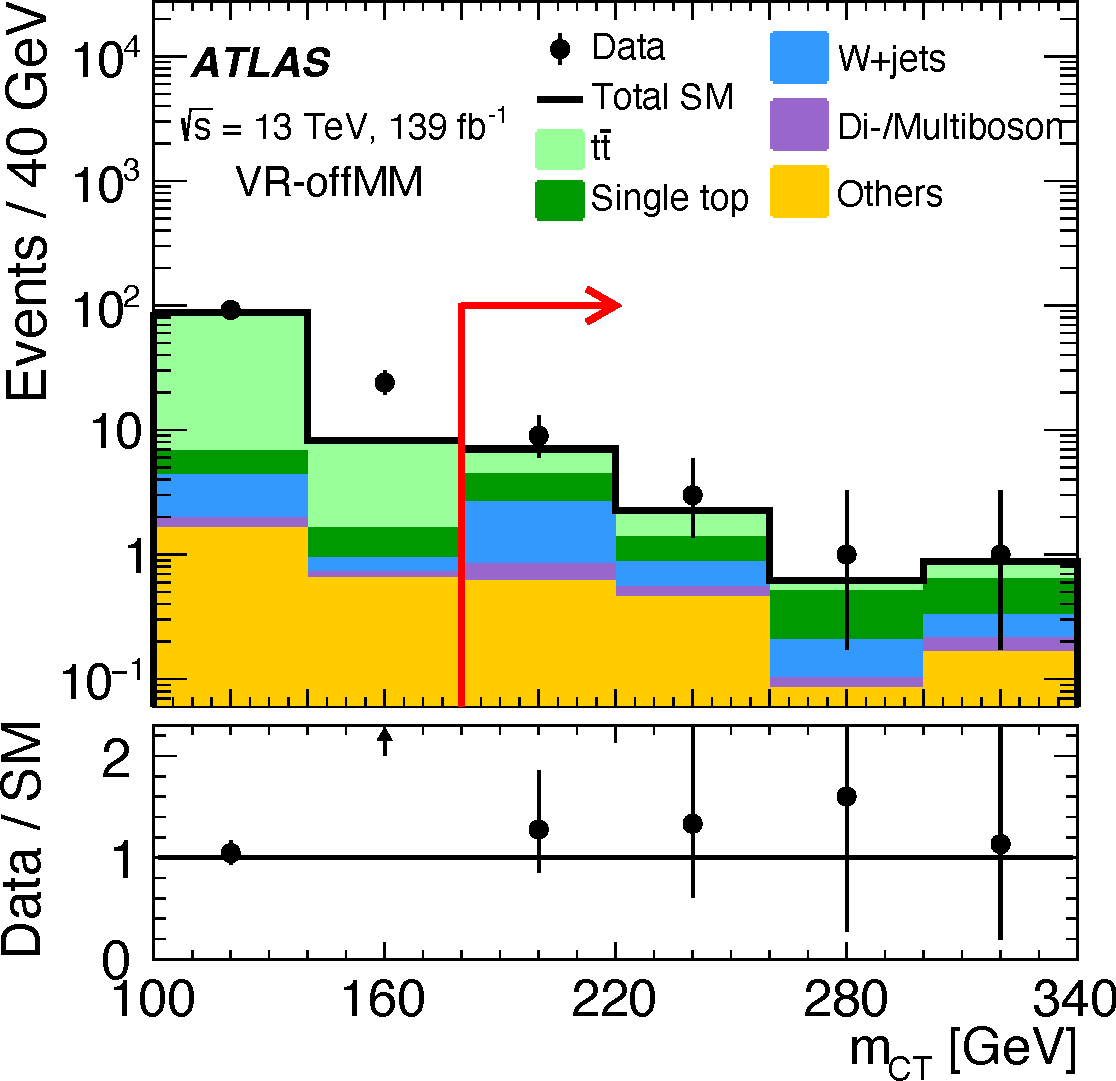
\includegraphics[width=0.85\textwidth]{OneLeptonbb_VR_UnderFlowBin_VRtt2offnomct2EM_mct2_yellow}
	\end{subfigure}\hfill
	\begin{subfigure}[b]{0.5\linewidth}
		\centering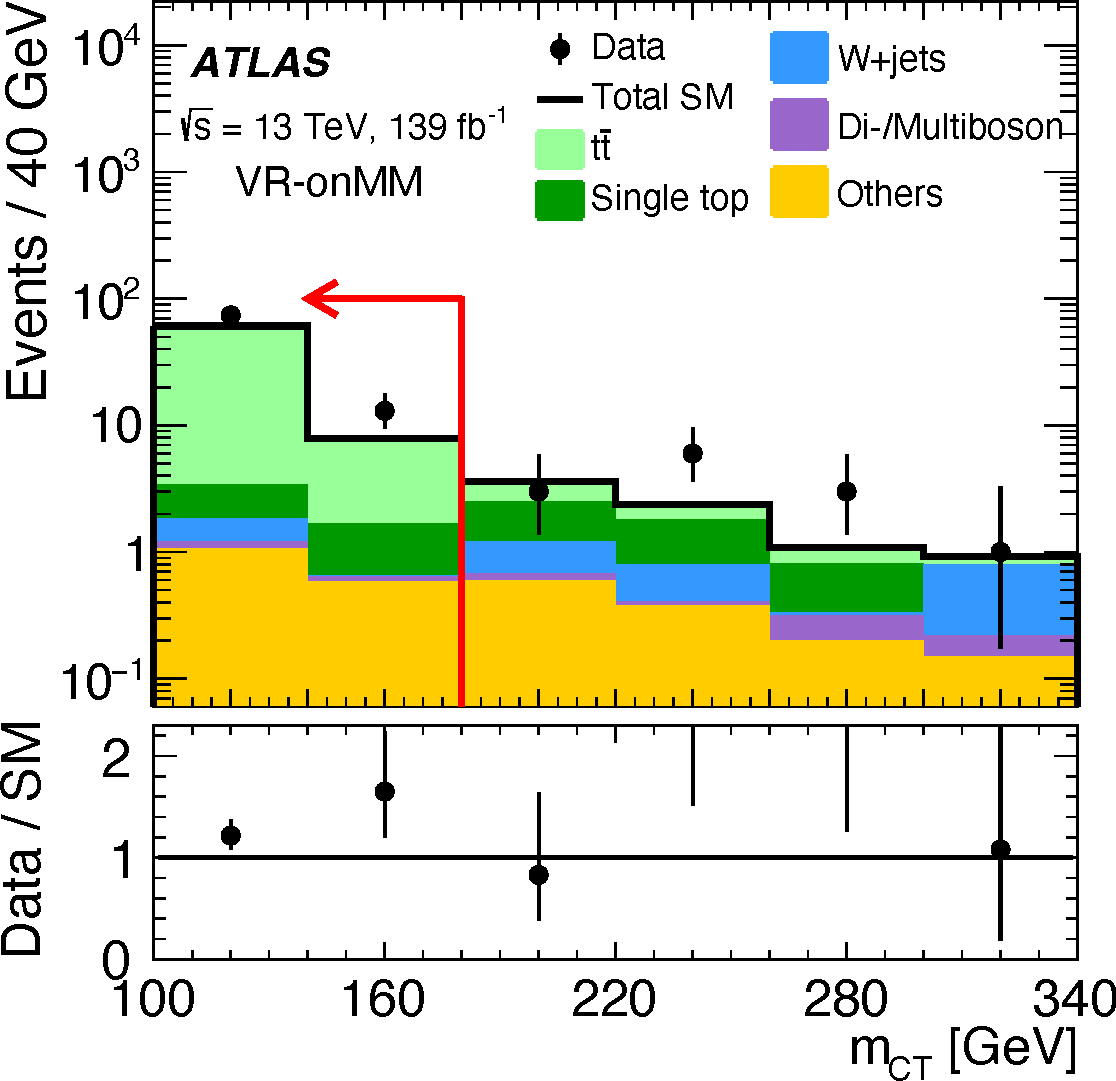
\includegraphics[width=0.85\textwidth]{OneLeptonbb_VR_UnderFlowBin_VRtt2onnomct2EM_mct2_yellow}
	\end{subfigure}\hfill
	\par\medskip
	\begin{subfigure}[b]{0.5\linewidth}
		\centering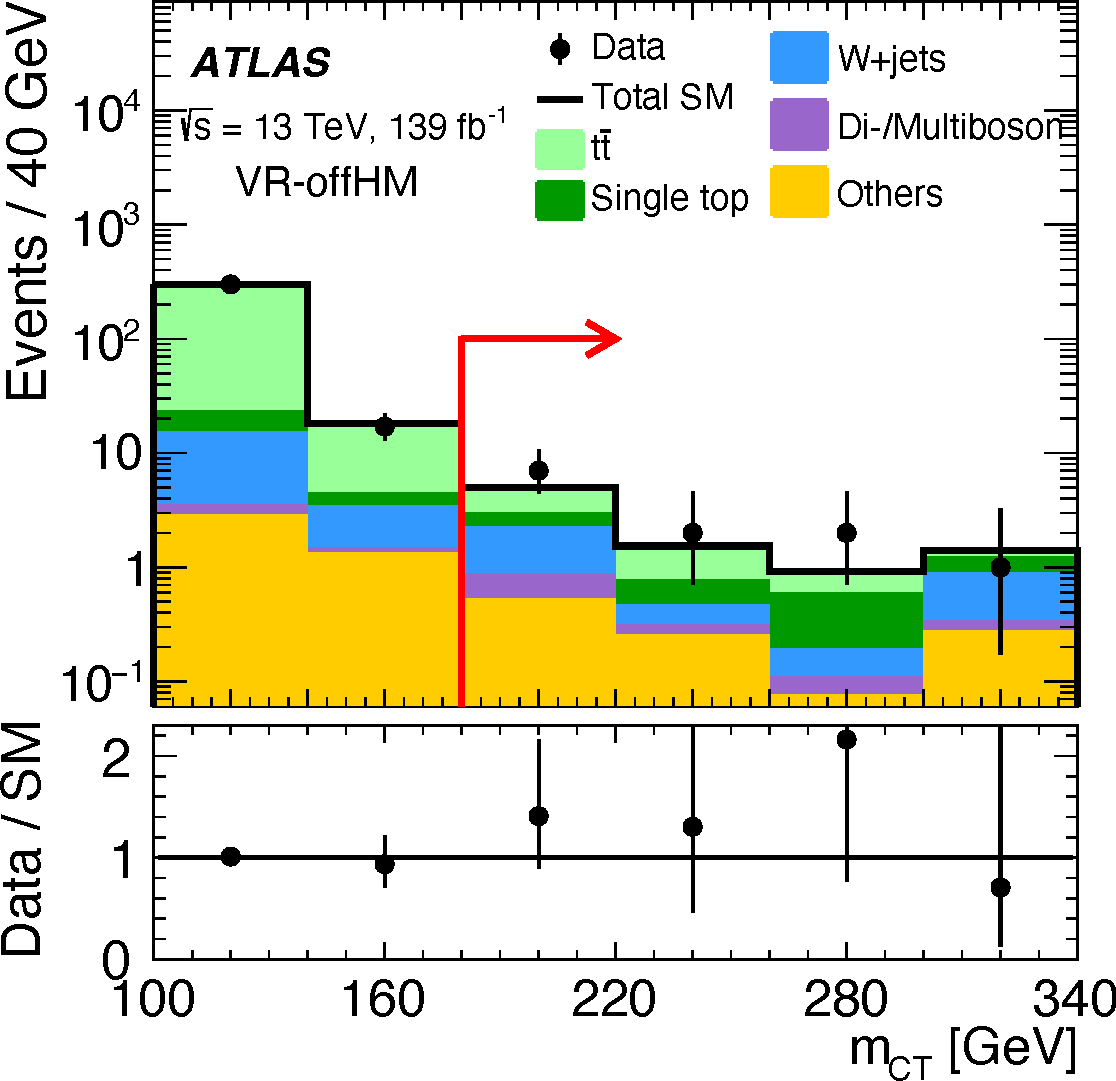
\includegraphics[width=0.85\textwidth]{OneLeptonbb_VR_UnderFlowBin_VRtt3offnomct2EM_mct2_yellow}
	\end{subfigure}\hfill
	\begin{subfigure}[b]{0.5\linewidth}
		\centering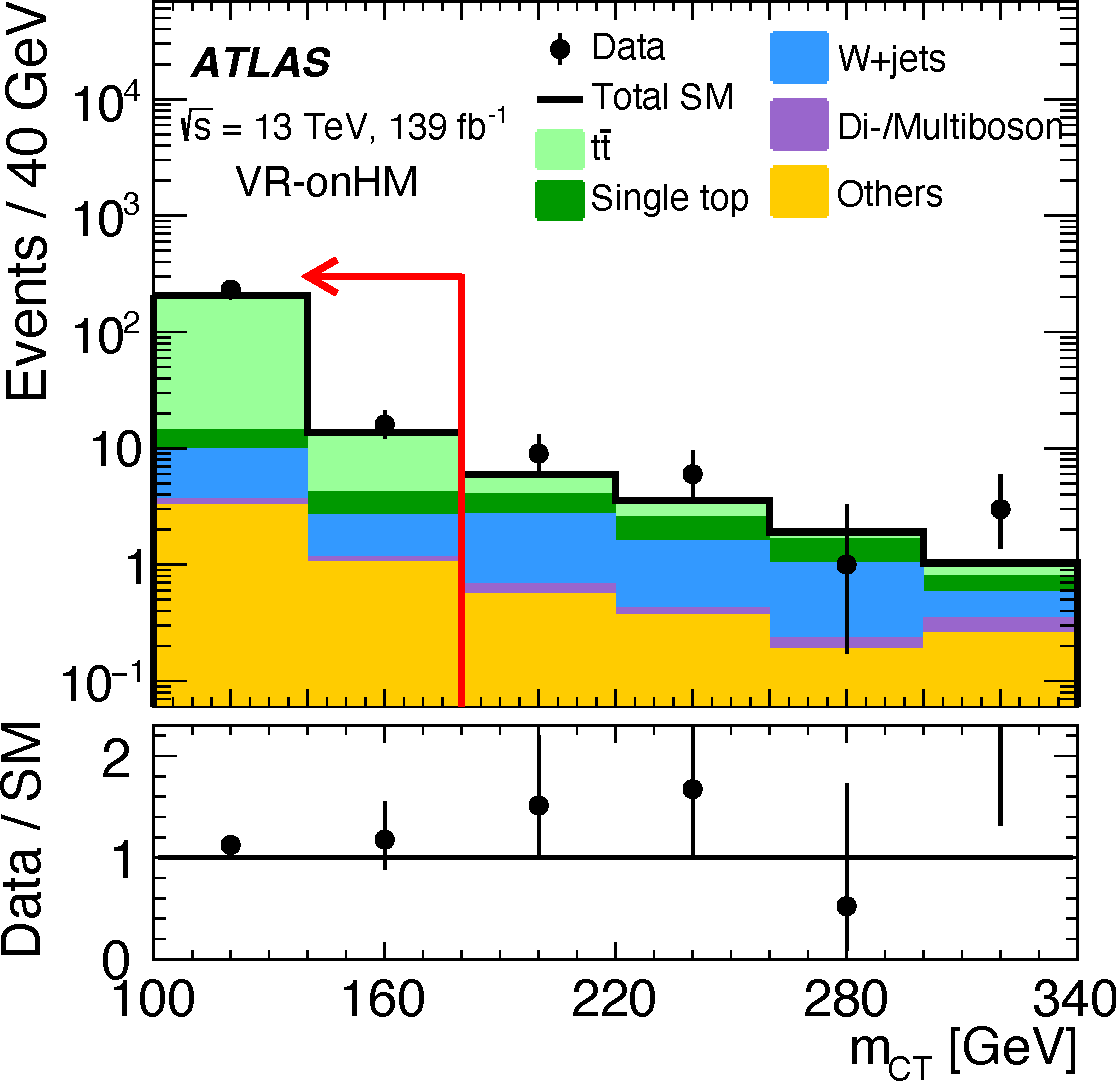
\includegraphics[width=0.85\textwidth]{OneLeptonbb_VR_UnderFlowBin_VRtt3onnomct2EM_mct2_yellow}
	\end{subfigure}\hfill

	\caption{Exemplary distributions shown in each validation region after the background-only fit with subsequent extrapolation to the \glspl{vr}. All selection cuts except for the requirement on $\mct$ (indicated using the red arrow) are applied. The shaded region includes all systematic uncertainties as well as \gls{mc} statistical uncertainty.}
	\label{fig:VR_distributions_postfit}
\end{figure}



\begin{table}
\begin{center}
{\small
%%
\begin{tabular}{lrrrrrr}
\toprule
Region      & VR-onLM            & VR-onMM            & VR-onHM     & VR-offLM            & VR-offMM            & VR-offHM              \\[-0.05cm]
\midrule
%%
Observed events      & $103$              & $87$              & $247$      & $27$              & $14$              & $12$                    \\
\midrule
%%
Fitted SM events    & $100 \pm 19$          & $64 \pm 9$          & $215 \pm 18$      & $34 \pm 6$          & $9.5 \pm 2.7$          & $7.5 \pm 2.6$              \\
\midrule
%%
       $\ttbar$      & $90 \pm 19$          & $59 \pm 9$          & $196 \pm 19$   & $18 \pm 4$          & $2.4 \pm 1.4$          & $1.8 \pm 1.8$              \\
%%
        Single top      & $5_{-5}^{+5}$          & $2.6_{-2.6}^{+2.9}$          & $6 \pm 6$     & $5 \pm 4$          & $3.0 \pm 1.8$          & $1.8 \pm 1.5$              \\
%%
        $\wjets$      & $4 \pm 4$          & $0.6 \pm 0.5$          & $7.9 \pm 2.1$     & $8.2 \pm 2.6$          & $2.3 \pm 0.8$          & $2.2 \pm 0.6$              \\
%%
        Di-/Multiboson       & $0.24 \pm 0.08$          & $0.19 \pm 0.08$          & $0.54 \pm 0.19$   & $1.07 \pm 0.27$          & $0.39 \pm 0.11$          & $0.51 \pm 0.14$              \\
%%
        Other       & $1.34 \pm 0.22$          & $1.67 \pm 0.28$          & $4.4 \pm 2.0$      & $1.6 \pm 0.5$          & $1.34 \pm 0.25$          & $1.15 \pm 0.24$              \\
%%     
\toprule
%%
MC exp. SM events     & $110 \pm 40$          & $69 \pm 17$          & $218 \pm 22$          & $34 \pm 7$          & $12.8 \pm 3.4$          & $9.7 \pm 3.3$              \\
\midrule
%%
        $\ttbar$           & $92 \pm 35$          & $62 \pm 17$          & $196 \pm 21$     & $16 \pm 5$          & $3.8 \pm 2.2$          & $3.1 \pm 1.9$              \\
%%
       Single top     & $8 \pm 5$          & $4.5 \pm 3.4$          & $11 \pm 6$    & $9 \pm 4$          & $5.3 \pm 2.2$          & $3.1 \pm 2.5$              \\
%%
        $\wjets$        & $2.8 \pm 2.3$          & $0.5 \pm 0.5$          & $6.5 \pm 1.2$    & $6.5 \pm 1.6$          & $2.0 \pm 0.5$          & $1.80 \pm 0.34$              \\
%%
        Di-/Multiboson       & $0.24 \pm 0.07$          & $0.19 \pm 0.08$          & $0.50 \pm 0.17$     & $1.07 \pm 0.28$          & $0.37 \pm 0.10$          & $0.50 \pm 0.15$              \\
%%
        Other       & $1.35 \pm 0.23$          & $1.70 \pm 0.28$          & $4.4 \pm 0.9$    & $1.6 \pm 0.5$          & $1.36 \pm 0.25$          & $1.16 \pm 0.24$              \\
%%     \\
\bottomrule
\end{tabular}
%%%%
}
\end{center}
\caption{ Background-only fit results from the \glspl{cr} extrapolated to the \glspl{vr} for an integrated luminosity of \onethirtynineifb. Nominal MC expectations (normalised to MC cross-sections) are given for comparison. The errors shown include the \gls{mc} statistical and systematic uncertainties. Uncertainties in the fitted event rates are symmetric by construction, except where the negative error is truncated at an event rate of zero.
%PDG rounding is applied to the event rates and uncertainties~\cite{pdg2020}.
}
\label{tab:results_bkg_only_VR}
\end{table}
%

In order to validate the extrapolations from the \glspl{cr} to the \glspl{sr}, the results of the background-only fit in the \glspl{cr} are extrapolated into the \glspl{vr}. \Cref{tab:results_bkg_only_VR} details the observed data and background estimation before and after the fit in the different \gls{vr} bins. 

In the on-peak \glspl{vr}, $\ttbar$ is by far the dominant background after the background-only fit. Contributions from single top and $\wjets$ each amount to only 1--5\%, depending on validation region bin. Diboson, multiboson and other \gls{sm} processes result in minor contributions of the level of not more than 3\% of the total background estimate. As the total uncertainties on the background estimate in the on-peak regions are dominated by the $\ttbar$ uncertainties, the large uncertainties on the $\wjets$ and single top estimate due to relatively limited \gls{mc} statistics do not have a significant impact. 
In the off-peak \glspl{vr} after the background-only fit, $\ttbar$ is the dominant process in the low mass regime, while contribution from single top and $\wjets$ are subdominant. In the medium and high mass regimes, $\ttbar$, single top and $\wjets$ all result in similar contributions. Diboson, multiboson and other \gls{sm} processes are only minor backgrounds in all off-peak regions, cumulatively amounting to only 10--14\% of the total background estimate, depending on the mass regime.
Exemplary $N-1$ distributions in the validation regions after the background-only fit are shown in~\cref{fig:VR_distributions_postfit}.

The agreement between data and the background estimate is summarised in~\cref{fig:result_histpull}. \improvement{quote exact numbers} The background estimates agree within $1.3\sigma$ with the observed data in all validation regions, except for VR-onMM where the agreement is within $1.7\sigma$. Thus, the overall agreement in the validation regions is considered to be acceptable, paving the way for further extrapolation of the background estimate into the \glspl{sr}.

\subsection{Results in the signal regions}

By extrapolating the results from the background-only fit in the control regions, the background estimate in the signal regions can be obtained. \Cref{tab:results_bkg_only_SR_disc} compares the background estimate with the observed data for all discovery signal regions. In the low mass discovery signal region, $\ttbar$ is the dominant background, followed by $\wjets$ and single top. In the medium mass discovery signal region, all three main backgrounds contribute at roughly equal parts. In the high mass signal region, $\wjets$ is the largest \gls{sm} background, followed by single top and $\ttbar$. In all discovery signal regions, diboson, multiboson and other \gls{sm} backgrounds yield only minor contributions. The results in the exclusion signal regions are shown in \cref{tab:results_bkg_only_SR}. As for the discovery signal regions, $\ttbar$ is the dominant background in the low mass signal region bins, while $\wjets$ slightly dominates in the high mass signal region bins. The $\mct$ distribution in all three exclusion \glspl{sr} are shown in~\cref{fig:SR_distributions_postfit}.

None of the exclusion or discovery signal regions reveal a significant deviation in data compared to the \gls{sm} expectation, meaning that all observations are compatible with the \gls{sm}. Consequently, the signal regions will be used in the following to derive model-dependent exclusion limits as well as model-independent upper limits. A slight overfluctuation of data in the discovery \glspl{sr} (that are not mutually exclusive) is quantified to be within $1.8\sigma$ in the inclusive SR-LM, resulting in weaker model-independent upper limits than expected. Some of the exclusion signal region bins also exhibit small overfluctuations in data. In SR-LM low $\mct$ (SR-HM low $\mct$), the overfluctuation in data amounts to $1.5\sigma$ ($1.3\sigma$) compared to the \gls{sm} expectation. The largest difference is seen in SR-MM medium $\mct$, however with a disagreement of only $1.6\sigma$, the observations in data are overall in good agreement with the \gls{sm} expectation. Due to the small excesses, however, the observed model-dependent exclusion limit derived in~\cref{sec:results_interpretation} is slightly weaker than expected. \Cref{fig:result_histpull} summarises across all regions the observed data, \gls{sm} background expectation as well as the significances of any deviations.



\begin{table}
\begin{center}
{\small
%%
\begin{tabular}{lrrr}
\toprule
Region           & SR-LM (disc.)           & SR-MM (disc.)           & SR-HM  (disc.)            \\
\midrule
%%
Observed events          & $66$              & $32$              & $14$                    \\
\midrule
%%
Fitted SM events         & $47 \pm 6$          & $21 \pm 5$          & $8.6 \pm 2.8$              \\
\midrule
%%
        $\ttbar$         & $22 \pm 4$          & $5.9 \pm 1.9$          & $1.9 \pm 0.7$              \\
%%
        Single top         & $9 \pm 6$          & $6 \pm 5$          & $2.0_{-2.0}^{+2.4}$              \\
%%
        $\wjets$         & $11.1 \pm 2.9$          & $5.6 \pm 1.4$          & $3.7 \pm 1.0$              \\
%%
        Di-/Multiboson         & $1.23 \pm 0.24$          & $0.56 \pm 0.11$          & $0.21 \pm 0.06$              \\
%%
        Other         & $4.8 \pm 0.5$          & $2.6 \pm 0.4$          & $0.74 \pm 0.16$              \\
%%     
\toprule
%%
MC exp. SM events              & $50 \pm 7$          & $22 \pm 5$          & $8 \pm 4$              \\
\midrule
%%
        $\ttbar$         & $21 \pm 5$          & $4.9 \pm 1.6$          & $1.2 \pm 0.6$              \\
%%
        Single top         & $14 \pm 4$          & $9 \pm 5$          & $2.9_{-2.9}^{+3.5}$              \\
%%
        $\wjets$         & $9.1 \pm 1.3$          & $4.5 \pm 0.7$          & $3.0 \pm 0.6$              \\
%%
        Di-/Multiboson         & $1.20 \pm 0.23$          & $0.56 \pm 0.11$          & $0.21 \pm 0.06$              \\
%%
        Other        & $4.8 \pm 0.5$          & $2.6 \pm 0.4$          & $0.74 \pm 0.16$              \\
%%     \\
\bottomrule
\end{tabular}
%%%%
}
\end{center}
\caption{ Background-only fit results extrapolated to the discovery \glspl{sr} for an integrated luminosity of \onethirtynineifb. Nominal MC expectations (normalised to MC cross-sections) are given for comparison. The errors shown include the \gls{mc} statistical and systematic uncertainties. Uncertainties in the fitted yields are symmetric by construction, except where the negative error is truncated at an event yield of zero. PDG rounding is applied to the event rates and uncertainties.}
\label{tab:results_bkg_only_SR_disc}
\end{table}
%

\begin{table}
\begin{center}
{\small
%%
\begin{tabular}{lrrrr}
\toprule
{\textbf{ SR-LM}}           & All $\mct$ bins          & Low $\mct$         & Medium $\mct$        & High $\mct$    \\[-0.05cm]
\midrule
Observed           & $34$              & $16$              & $11$              & $7$                    \\
\midrule
Expected          & $27 \pm 4~~$          & $8.8 \pm 2.8$          & $11.3 \pm 3.1~~$          & $7.3 \pm 1.5$              \\
\midrule
$\ttbar$          & $16.2 \pm 3.4~~$          & $4.4 \pm 2.2$          & $7.3 \pm 2.5$          & $4.6 \pm 1.2$              \\
Single top          & $2.7 \pm 1.8$          & $1.3 \pm 1.1$          & $0.9_{-0.9}^{+1.0}~$          & $0.6 \pm 0.6$              \\
$W$+jets           & $5.5 \pm 2.0$          & $2.0 \pm 0.9$          & $2.4 \pm 1.3$          & $1.1 \pm 0.5$              \\
Di-/Multiboson          & $0.67 \pm 0.19$          & $0.39 \pm 0.13$          & $0.09_{-0.09}^{+0.11}~$          & $0.18 \pm 0.04$              \\
Others          & $2.23 \pm 0.29$          & $0.81 \pm 0.25$          & $0.64 \pm 0.15$          & $0.77 \pm 0.12$              \\
\bottomrule
\textbf{ SR-MM}           & All $\mct$ bins          & Low $\mct$         & Medium $\mct$        & High $\mct$    \\[-0.05cm]
\midrule
Observed           & $13$              & $4$              & $7$              & $2$                    \\
\midrule
 Expected          & $8.6 \pm 2.2$          & $4.6 \pm 1.7$          & $2.6 \pm 1.3$          & $1.4 \pm 0.6$              \\
\midrule
$\ttbar$          & $2.7 \pm 1.4$          & $1.6 \pm 0.9$          & $0.8 \pm 0.7$          & $0.30 \pm 0.24$              \\
Single top          & $2.7 \pm 1.9$          & $1.6 \pm 1.5$          & $1.0_{-1.0}^{+1.1}~$          & $0.15_{-0.15}^{+0.19}~$              \\
$W$+jets          & $1.5 \pm 0.7$          & $0.6 \pm 0.4$          & $0.3_{-0.3}^{+0.4}~$          & $0.57 \pm 0.26$              \\
Di-/Multiboson          & $0.29 \pm 0.08$          & $0.09 \pm 0.04$          & $0.065 \pm 0.028$          & $0.14 \pm 0.06$              \\
Others          & $1.33 \pm 0.27$          & $0.69 \pm 0.20$          & $0.40 \pm 0.13$          & $0.24 \pm 0.09$              \\
\bottomrule
\textbf{ SR-HM}           & All $\mct$ bins          & Low $\mct$         & Medium $\mct$        & High $\mct$    \\[-0.05cm]
\midrule
Observed           & $14$              & $6$              & $5$              & $3$                    \\
\midrule
 Expected          & $8.1 \pm 2.7$          & $4.1 \pm 1.9$          & $2.9 \pm 1.3$          & $1.1 \pm 0.5$              \\
\midrule
         $\ttbar$          & $1.4 \pm 0.5$          & $0.8 \pm 0.4$          & $0.36 \pm 0.25$          & $0.22 \pm 0.15$              \\
Single top          & $2.0_{-2.0}^{+2.4}~$          & $0.9_{-0.9}^{+1.5}~$         & $0.9 \pm 0.9$          & $0.16_{-0.16}^{+0.26}~$              \\
$W$+jets           & $3.7 \pm 1.0$          & $1.9 \pm 0.8$          & $1.4 \pm 0.8$          & $0.45 \pm 0.19$              \\
Di-/Multiboson          & $0.21 \pm 0.06$          & $0.057 \pm 0.025$          & $0.075 \pm 0.027$          & $0.08 \pm 0.04$              \\
Others          & $0.74 \pm 0.16$          & $0.34 \pm 0.09$          & $0.19 \pm 0.08$          & $0.21 \pm 0.08$              \\
\bottomrule
\end{tabular}
}
\end{center}
\caption{ Background-only fit results in the exclusion \glspl{sr} for an integrated luminosity of \onethirtynineifb. The first column shows the sum of all $\mct$ bins. Subsequent columns indicate the different bins in $\mct$, the overflow is included in the last bin. The errors shown include the \gls{mc} statistical and systematic uncertainties. Uncertainties in the fitted yields are symmetric by construction, except where the negative error is truncated at an event yield of zero.
%PDG rounding is applied to the event rates and uncertainties~\cite{pdg2020}.
Table adapted from \reference\cite{SUSY-2019-08}.}\label{tab:results_bkg_only_SR}
\end{table}
%


 \begin{figure}
	\centering
	\begin{subfigure}[b]{0.5\linewidth}
		\centering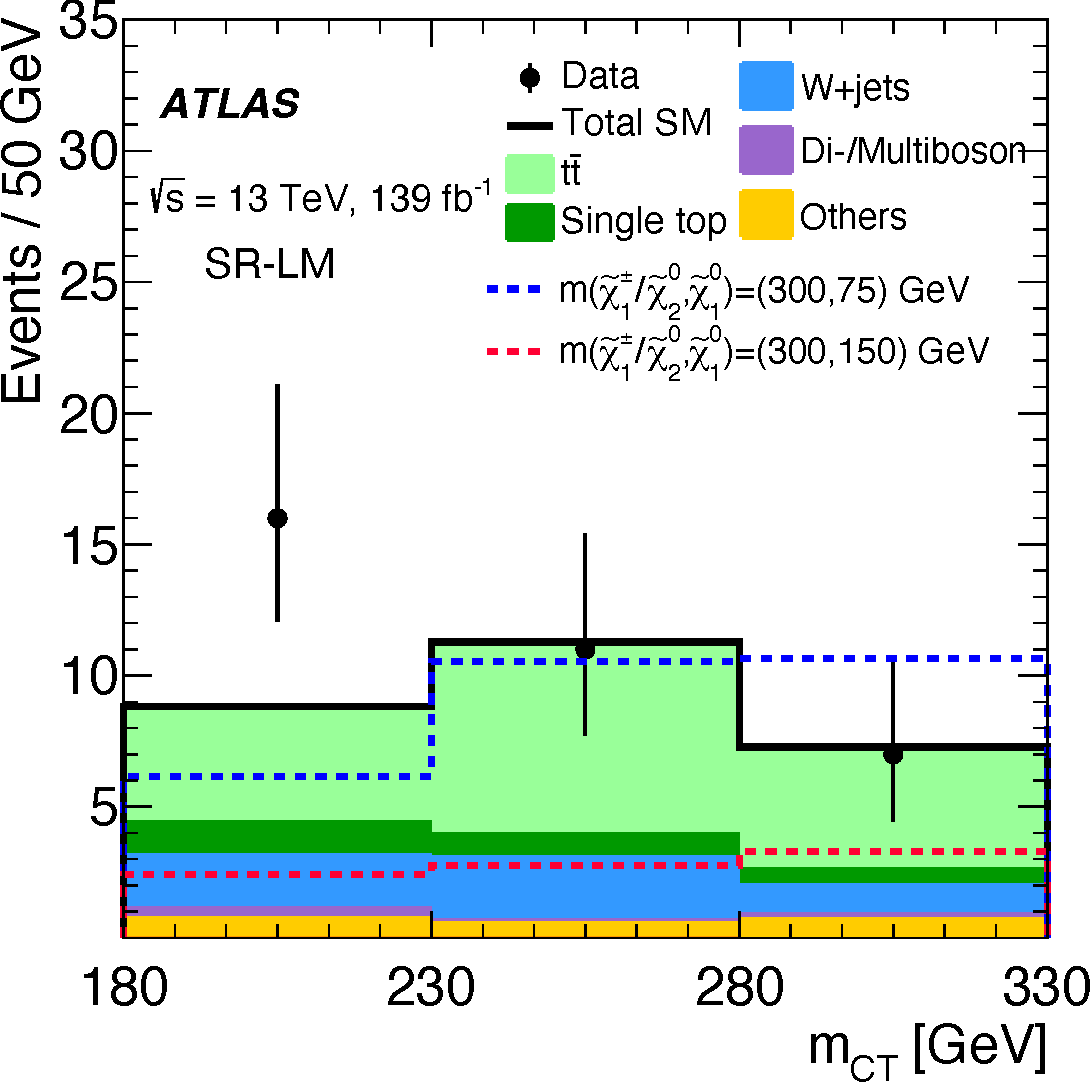
\includegraphics[width=0.85\textwidth]{OneLepton_Wh_SRLMEM_mct2_yellow}
	\end{subfigure}\hfill
	\begin{subfigure}[b]{0.5\linewidth}
		\centering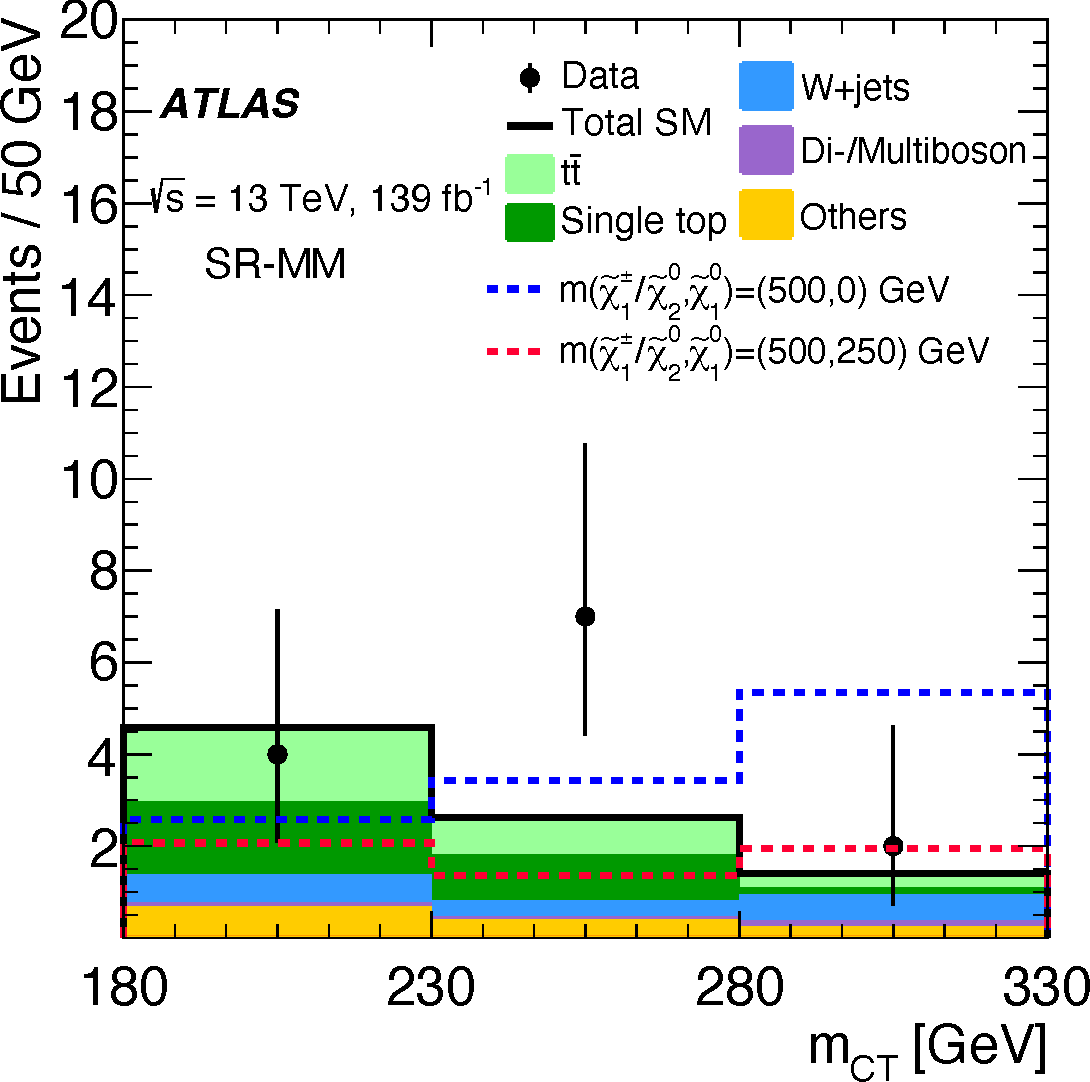
\includegraphics[width=0.85\textwidth]{OneLepton_Wh_SRMMEM_mct2_yellow}
	\end{subfigure}\hfill
	\begin{subfigure}[b]{0.5\linewidth}
		\centering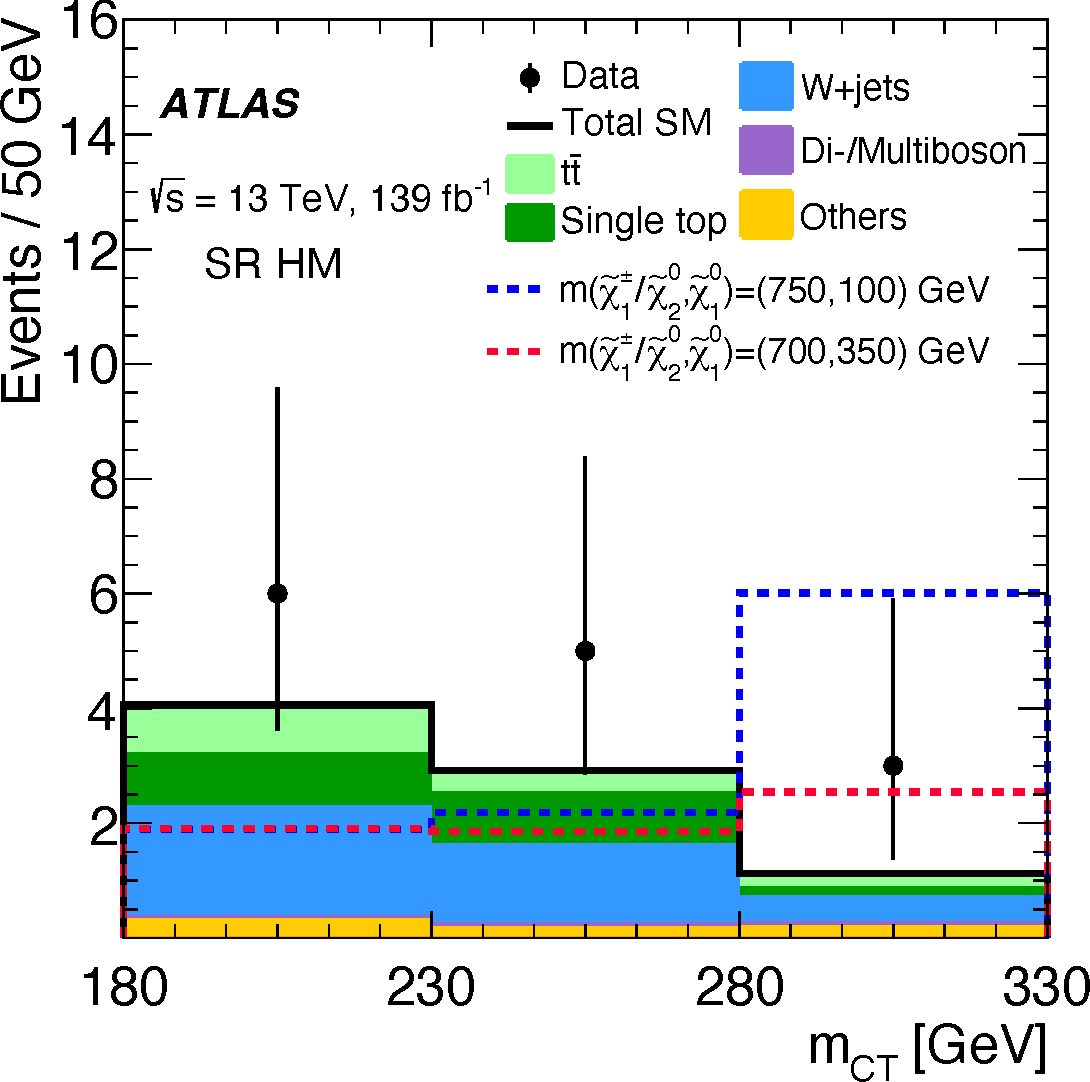
\includegraphics[width=0.85\textwidth]{OneLepton_Wh_SRHMEM_mct2_yellow}
	\end{subfigure}\hfill

	\caption{Exemplary distribution shown in each exclusion signal region after the background-only fit. The shaded region includes all systematic uncertainties (including correlations) as well as \gls{mc} statistical uncertainty.}
	\label{fig:SR_distributions_postfit}
\end{figure}


 \begin{figure}
	\centering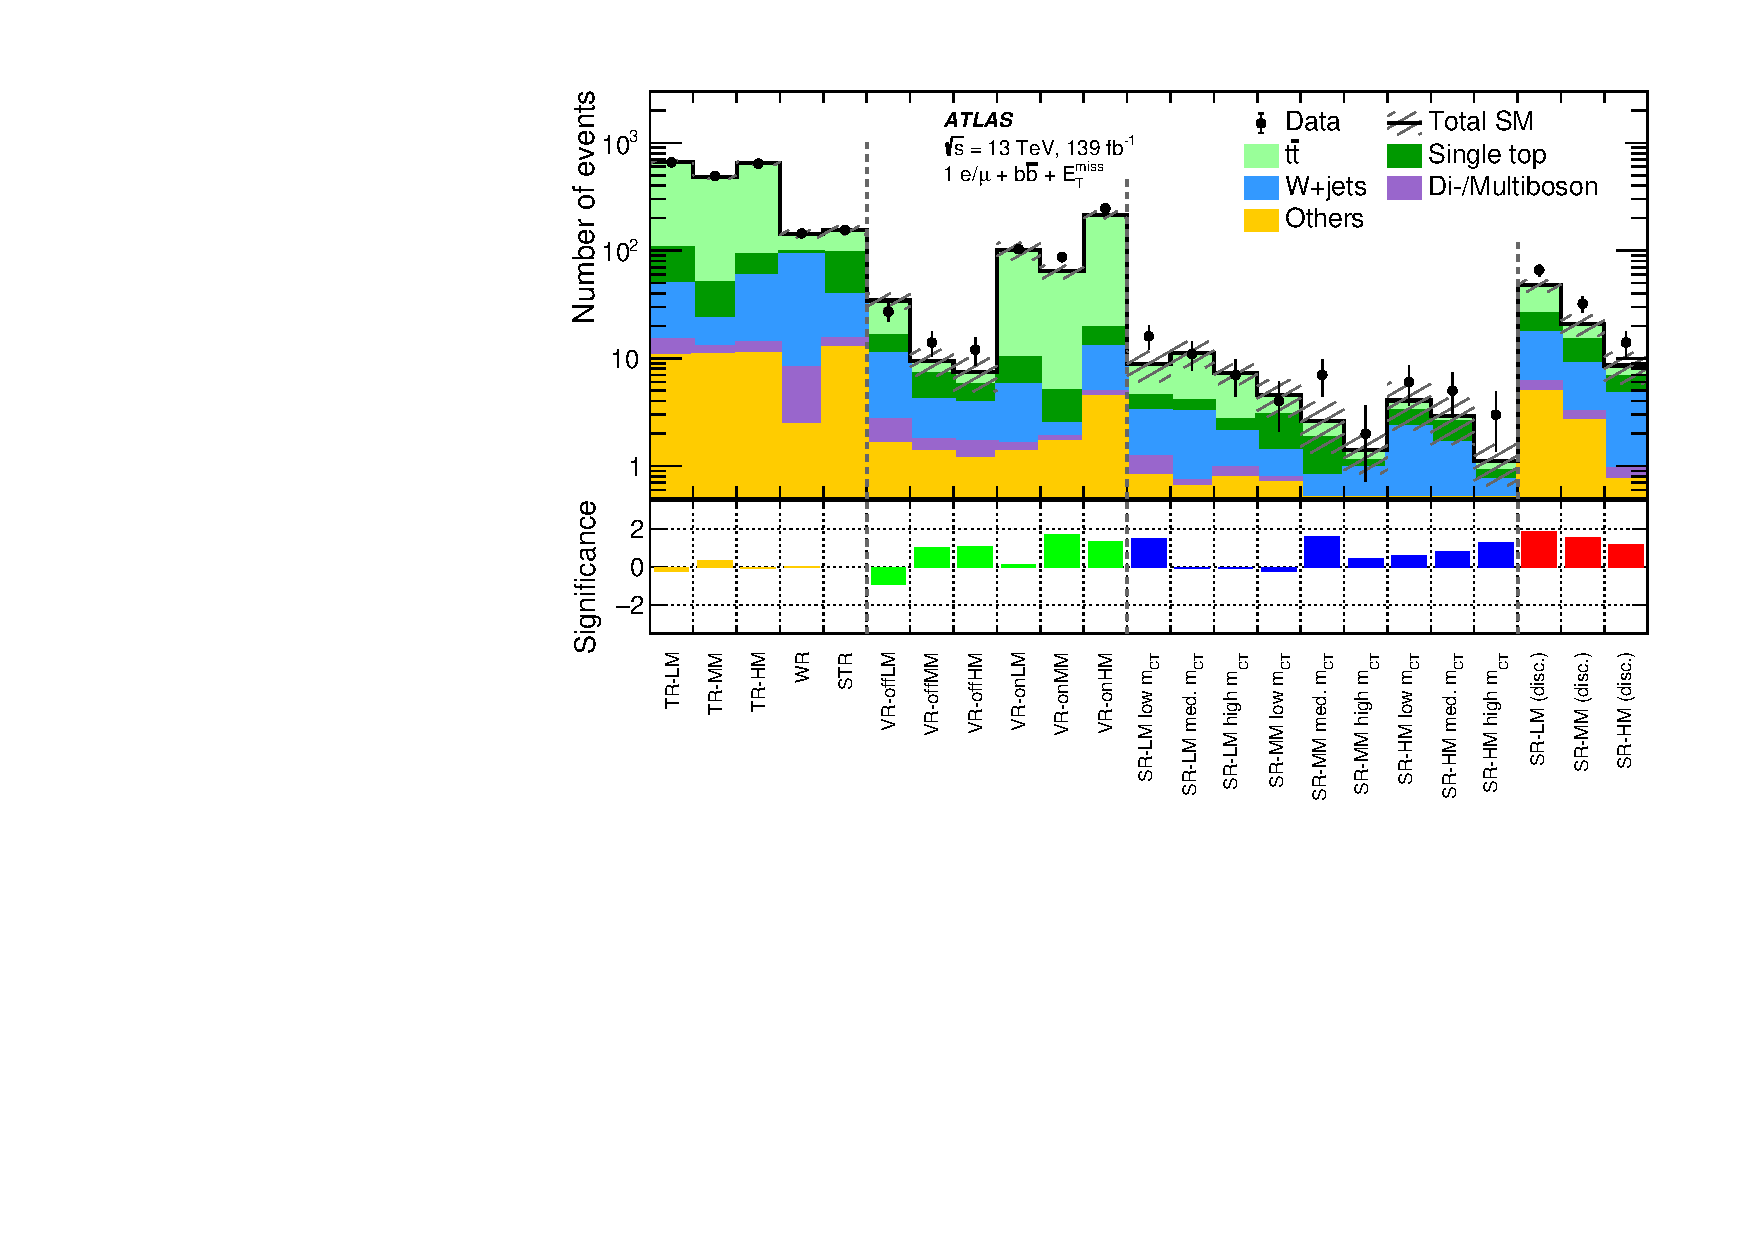
\includegraphics[width=0.95\textwidth]{histpull_CRVRSR}
	\caption{Comparison of the observed data and expected event rates in all regions considered in the analysis. The shaded uncertainty band includes both \gls{mc} statistical and systematic uncertainties. The significances~\cite{Cousins:2007bmb} of the differences between the observed data and expected event rates are shown in the bottom panel. The discovery signal regions are not statistically independent from each other, nor from the exclusion signal regions.}
	\label{fig:result_histpull}
\end{figure}


\FloatBarrier

\section{Interpretation}\label{sec:results_interpretation}

As no significant excess of data is observed in any of the signal regions, model-independent upper limits as well as model-dependent exclusion limits are computed.

\subsection{Model-independent upper limits} 

Model-independent upper limits on the visible cross section of new physics processes are derived using the discovery \glspl{sr}. For this, a likelihood containing terms for the \glspl{cr} and the discovery \glspl{sr} is used. Since the discovery \glspl{sr} are not mutually exclusive, only one discovery \gls{sr} enters the likelihood at a time. This results in three distinct fit configurations in which the signal strength $\mu$ is the \gls{poi} and no signal contamination is assumed in the control regions. The \gls{poi} is subsequently scanned in distinct steps from 0 to high\footnote{The signal strength is in principle allowed to exceed unity in order for the scan to find a 95\% CL upper limit} values, followed by a hypothesis test at each scan step. The upper limit on the number of observed signal events $S_{\mathrm{ obs}}^{95}$ is then given by the value of $\mu$ for which the corresponding CL$_s$ value drops below 0.05. An upper limit on the visible cross section $\langle\epsilon{\mathrm{ \sigma}}\rangle_{\mathrm{ obs}}^{95}$ is obtained by dividing $S_{\mathrm{ obs}}^{95}$ by the integrated luminosity of \onethirtynineifb. In addition to the upper limits on $\langle\epsilon{\mathrm{ \sigma}}\rangle_{\mathrm{ obs}}^{95}$ and $S_{\mathrm{ obs}}^{95}$,~\cref{tab:upperlimit_toys} also gives the $p$-values (and corresponding significances) for rejecting the background-only hypothesis in favour of the signal-plus-background hypothesis. As all significances are below $1.88\sigma$ for all \glspl{sr}, the background-only hypothesis cannot be rejected.

\begin{table}
\begin{center}
%\resizebox{\textwidth}{!}{
\begin{tabular}{lcccccc}
\toprule
\textbf{Signal Region}                       & $\langle\epsilon{\mathrm{ \sigma}}\rangle_{\mathrm{ obs}}^{95}$[fb]  &  $S_{\mathrm{ obs}}^{95}$  & $S_{\mathrm{ exp}}^{95}$ & $\textrm{CL}_{\textrm{B}}$ & $p_{0}$ & $Z$  \\
\midrule
 SR-LM $\mathrm{(disc.)}$    & $0.26$ &  $36.8$ & $ { 20.0 }^{ +8.0 }_{ -5.4 }$ & $0.97$ & $ 0.03$&$1.88$ \\%
 SR-MM $\mathrm{(disc.)}$    & $0.18$ &  $24.8$ & $ { 15.3 }^{ +6.2 }_{ -4.6 }$ & $0.94$ & $ 0.06$&$1.54$ \\%
 SR-HM $\mathrm{(disc.)}$    & $0.11$ &  $14.7$ & $ { ~~9.7 }^{ +3.3 }_{ -2.7 }$ & $0.89$ & $ 0.10$&$1.30$ \\%

\bottomrule
\end{tabular}
%}
\caption[Breakdown of upper limits.]{
The 95\% CL upper limits on the visible cross-section ($\langle\epsilon\sigma\rangle_{\mathrm{ obs}}^{95}$) and on the number of
signal events ($S_{\mathrm{ obs}}^{95}$) are given. Additionally, the expected 95\% CL upper limits on the number of signal events if no BSM signal is present ($S_{\mathrm{ exp}}^{95}$) are given, including their $\pm 1\sigma$ excursions. The last three columns indicate the confidence level observed for the background-only hypothesis ($\textrm{CL}_{\textrm{B}}$), the discovery $p$-value ($p_{0}$) and the significance $Z$~\cite{Cousins:2007bmb}.}
\label{tab:upperlimit_toys}
\end{center}
\end{table}


\subsection{Model-dependent exclusion limits}

For each signal point in the signal grid considered, a separate \textit{exclusion} fit is run using all \glspl{cr} and exclusion \glspl{sr}. As all exclusion signal region bins are disjoint, a likelihood containing terms for all bins can be constructed, effectively creating a shape-fit in the binned variables $\mt$ and $\mct$ (see \cref{ch:signal_region_optimisation}). As opposed to the background-only fit, the exclusion fits allow for signal contribution in all regions considered, and considers the signal strength $\mu$ to be a free parameter. For each point in the signal grid, the expected and observed CL$_s$ value is calculated as discussed in~\cref{sec:cls_approach}. Expected (observed) contour lines can then be drawn at expected (observed) CL$_s =0.05$. Signal points inside the contour are excluded at 95\% CL. \Cref{fig:result_exclusion} shows the exclusion contours obtained in the $\charg\neutr$ signal grid considered in the analysis. The dashed line corresponds to the expected exclusion contour, obtained using the Asimov dataset. The yellow uncertainty band represents the interval containing 68\% of all exclusion contours obtained for observations distributed according to the background-only hypothesis. The solid red line represents the observed exclusion limit obtained using the data recorded by ATLAS. As discussed in~\cref{sec:signal_theory_uncertainties}, the dashed red lines are obtained by varying the signal cross sections up and down by $1\sigma$.

Due to the slight overfluctuations of data observed in some of the exclusion signal region bins, the observed limit is slightly weaker than the expected one. The observed exclusion limit extends to about $\SI{740}{\GeV}$ in $m(\charg/\neutr)$ for massless $\lsp$, and up to $\SI{600}{\GeV}$ for $m(\lsp)=\SI{250}{\GeV}$. This extends the previous limit set by ATLAS in this simplified model and decay channel by more than $\SI{200}{\GeV}$ in $m(\charg/\neutr)$ for massless $\lsp$, an improvement made possible not only by the increase in integrated luminosity but also the introduction of a two-dimensional shape fit in the analysis strategy. 

 \begin{figure}
	\centering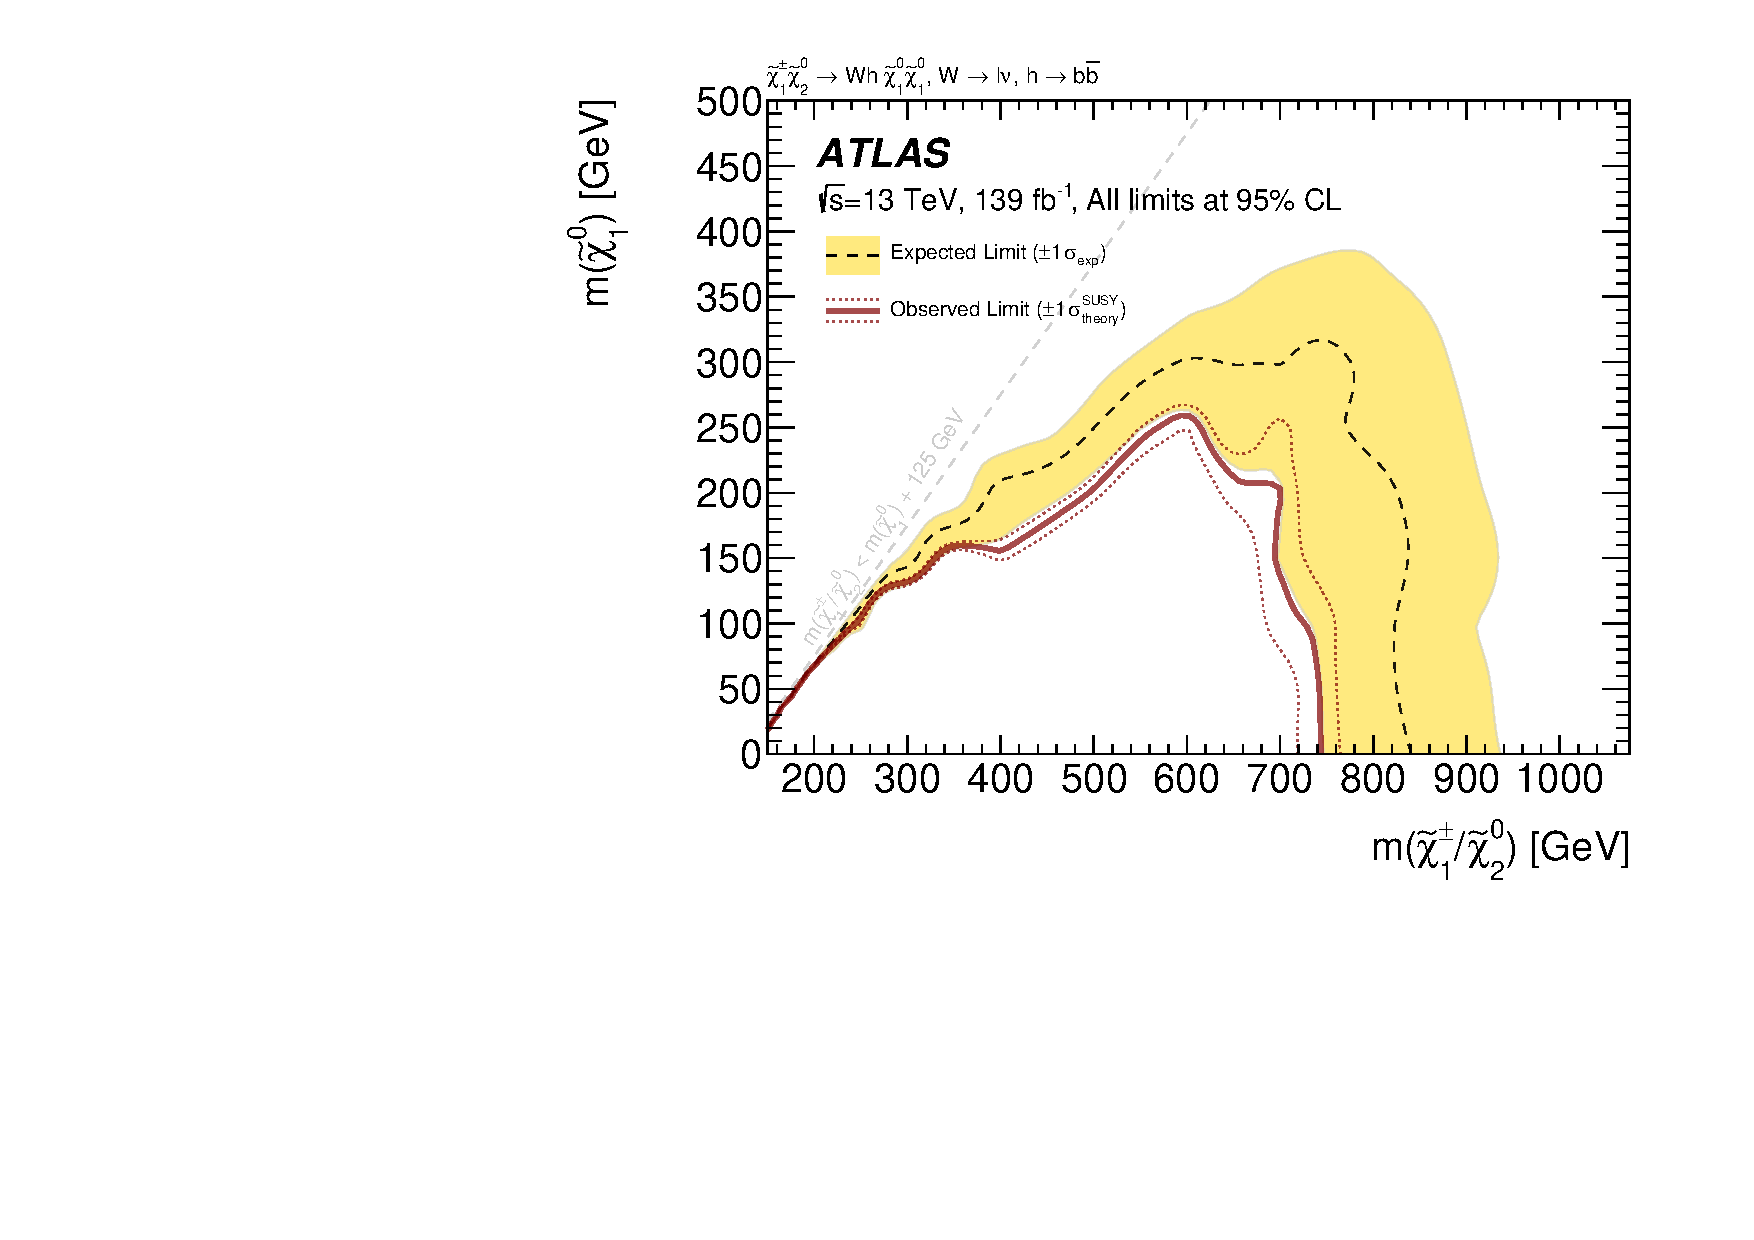
\includegraphics[width=0.75\textwidth]{contourPlotterWh1Lbb}
	\caption{Model-dependent exclusion contour on $\charg/\neutr$ pair production. The dashed black line represents the expected limit obtained using Asimov data. The uncertainties are given by the yellow band. The red solid line represents the observed limit obtained using \onethirtynineifb of data taken by ATLAS. By varying the signal cross sections up and down by their uncertainty, the red dashed lines are obtained. All contours are given at 95\% CL. }
	\label{fig:result_exclusion}
\end{figure}


\section{Discussion}

At the time of writing, the limits derived in this analysis are the most stringent limits on the $\charg\neutr\rightarrow Wh\lsp\lsp$ simplified model set by an ATLAS search~\cite{ATL-PHYS-PUB-2020-020}, surpassing not only the previous iteration of the analysis~\cite{SUSY-2017-01}, but also yielding more stringent limits than those published by ATLAS in other decay channels of the same model. \Cref{fig:result_wh_summary} shows a summary of results published by ATLAS searches in the $\charg\neutr\rightarrow Wh\lsp\lsp$ simplified model. The search presented in this work is referred to as \textit{1Lbb}. Additional searches in the $0\ell$ as well as \onelepton final states are being worked on, and are expected to extend the limits on $m(\charg/\neutr)$ up to roughly $\SI{1}{\TeV}$ for massless $\lsp$ as well as slightly extend the excluded parameter space towards the diagonal where $m(\charg/\neutr) = m(\lsp) + m(h)$\footnote{Assuming that no significant excess in data is seen in the search regions of these analyses.}.\improvement{cite}

 \begin{figure}
	\centering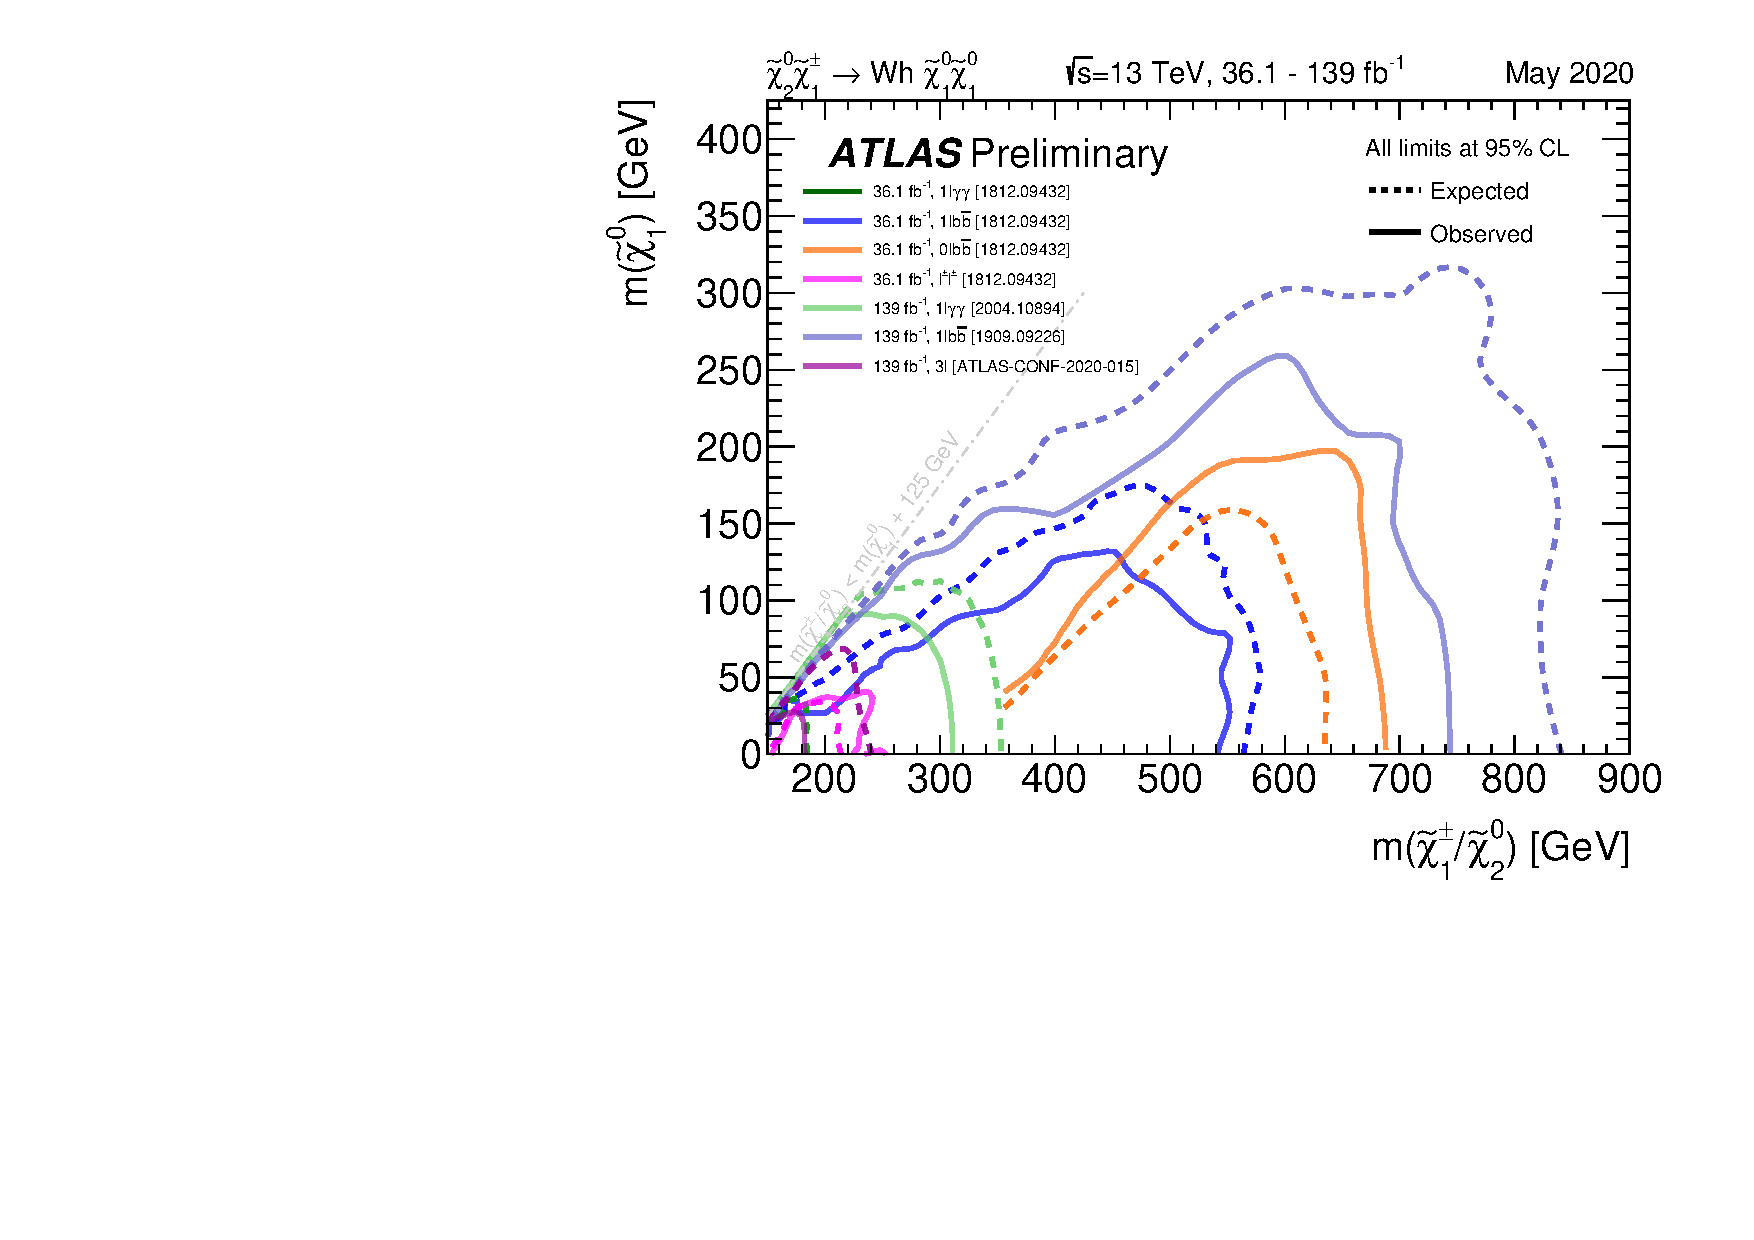
\includegraphics[width=0.75\textwidth]{fig_15}
	\caption{Summary of ATLAS limits on $\charg/\neutr$ masses in the $\charg\neutr\rightarrow Wh\lsp\lsp$ simplified model. The exclusion limit obtained by the analysis presented in this work is referred to as \textit{1Lbb} (the \onethirtynineifb iteration) and is the most stringent limit in this simplified model set by an ATLAS search thus far.}
	\label{fig:result_wh_summary}
\end{figure}

Various other searches for \gls{susy} at both ATLAS and CMS are constraining a multitude of other supersymmetric particle production and decay processes. The limits on gluino and squark pair production at the \gls{lhc} are particularly heavily constrained, reaching $\SI{2}{\TeV}$ in many cases. With the large integrated luminosity available through the full Run~2 dataset and the improved analysis techniques and strategies developed over the last years, the typically weaker limits on electroweakinos and sleptons are also significantly increasing and in some cases approach the $\SI{1}{\TeV}$ mark. The diverse \gls{susy} search programs at ATLAS and CMS thus heavily constrains the existence of \gls{susy} at the $\SI{}{\TeV}$ scale. 
Still, discarding the possibility for \gls{susy} to exist at the energies available with the \gls{lhc} is much too early, for several reasons. By the end of the lifetime of the \gls{lhc} (including the high luminosity upgrade HL-LHC), a projected amount of $\SI{3000}{\per\femto\barn}$~\cite{Apollinari:2116337} will have been delivered to the particle physics experiments. 
Many supersymmetric models not accessible with the full Run~2 dataset using today's analyses will hence only be in reach in the coming years of the \gls{lhc}.
%Finally, even if not directly accessible at LHC energies, \gls{susy} could reveal itself through quantum correction effects in precision measurements.

More importantly however, most of the quoted limits assume simplified \gls{susy} models and are thus only valid if the assumptions of the respective simplified model are realised in nature. 
In any realistic \gls{susy} scenario that could be realised in nature and is accessible to the \gls{lhc}, assumptions like 100\% branching ratios or a small set of supersymmetric particles participating in the decay chains are most likely not exactly fulfilled. 
Thus, the quoted simplified model limits can in general not be trivially interpreted as the true underlying constraint on the respective parameter of a more realistic \gls{susy} scenario. 
Due to the optimistic assumptions like 100\% branching fractions, the true constraints will in general be significantly weaker than the simplified model limits.
Reinterpretations of Run~1 ATLAS \gls{susy} searches in the \gls{pmssm}~\cite{pMSSM-scan-run1:2015baa} have indeed shown that constraints on the supersymmetric masses are weaker in more complex \gls{susy} models than those quoted for the simplified models studied in most analyses.

Naturally, there is a large interest in the high-energy physics community---both within ATLAS as well as outside of the collaboration---to perform reinterpretations of the existing \gls{susy} searches in new, promising signal models. Compelling reasons for performing reinterpretations include, amongst others, the possibility to state a combined sensitivity of the ATLAS search program to more realistic and complex \gls{susy} scenarios (compared to the simplified model limits). However, especially when considering high-dimensional parameter spaces like the \gls{pmssm}, such reinterpretation efficiencies quickly become extremely computationally expensive and require appropriate approximations. The following part of this work will introduce and discuss some of these approximations and show preliminary reinterpretation results of the analysis in the \gls{pmssm}.


